%             Exemple d'utilisation de la classe thesul
%             ------------------------------------------
%
%
% (de manière generale, les commandes de thesul sont celles
% qui ne sont pas complètement en minuscules)
%
% Voir la documentation complète pour plus de détails.
%   
%
% D. Roegel, 30 mars 2013
%
% \documentclass[12pt, oneside]{TUL/thesul}
\documentclass[12pt]{TUL/thesul}
%----------------------------------------------------------------------
%                     Chargement de quelques packages
%----------------------------------------------------------------------

% Si l'on veut produire une version PDF avec des hyperliens :
% \usepackage[pageanchor=false]{TUL/tulhypref}
% \usepackage[hidelinks, pdftex]{TUL/tulhypref}
\usepackage[hidelinks]{TUL/tulhypref}
% \usepackage[sc]{mathpazo}
\linespread{1.0}
% Si on veut le style de bibliographie named :
%\usepackage{named}

% Pour les figures :
\usepackage{graphicx}

% Si on veut des mini-tables des matières (utiliser minitoc-hyper 
% en conjonction avec tulhypref) :
\usepackage[french]{minitoc}

\usepackage{titlesec}
\usepackage{url}
\usepackage{listings}
\usepackage{pstricks}
\usepackage{subfigure}
\usepackage{amsmath}
\usepackage{amsthm}
\usepackage{amssymb}
\usepackage{tabularx}
\usepackage{textcomp}
\usepackage{multirow}
\usepackage[algoruled,french,onelanguage,algochapter]{algorithm2e}
\usepackage[section]{placeins}
\usepackage{xcolor}
\usepackage{colortbl}

\usepackage{epstopdf}
\usepackage{graphicx} % pour insérer des images
\usepackage{stmaryrd}
\usepackage{amsfonts}
% \usepackage{tikz}
% \usepackage{tikz-qtree}
% les figure imbriquées
\usepackage{epsfig}
% \usepackage{enumerate}

\usepackage{pgf}
\usepackage{tikz, calc}
% \usepackage{tikz-cd}
\usetikzlibrary{positioning}
\usetikzlibrary{fit}
\usetikzlibrary{shapes.multipart,calc}
\usetikzlibrary{arrows}

% \usepackage[math]{iwona} 
% \usepackage{iwona} 
% \SetMathAlphabet{\mathtt}{iwona}{OT1}{\ttdefault}{m}{n}

\usepackage[backend=biber, language=french, maxnames=5, citestyle=alphabetic,bibstyle=alphabetic,backref,abbreviate=false,dateabbrev=false,isbn=false,url=false,doi=true]{biblatex}
% \usepackage[backend=biber, language=french, maxnames=5,backref,abbreviate=false,dateabbrev=false,isbn=false,url=false,doi=true]{biblatex}
\addbibresource{these.bib}
% \usepackage[font=small,skip=0pt]{caption}
\usepackage[skip=0pt]{caption}
\usepackage{etoolbox}
\usepackage{needspace}

% Todo
\newcommand{\done}[1]{\todo[color=green!80!blue!80]{#1}}
\newcommand{\idone}[1]{\todo[inline,color=green!80!blue!80]{#1}}

% Samples
\newcommand{\telock}{tELock}

% Structure
\newtheorem{pb}{Problème}
\newtheorem{theo}{Théorème}
\newtheorem{defi}{Définition}
\newtheorem{prop}{Proposition}
\newtheorem{propri}{Propriété}
\newtheorem{pr}{Preuve}
\newtheorem{cor}{Corollaire}
\newtheorem{rem}{Remarque}
% \theoremstyle{remark}\newtheorem*{preuve}{Preuve}

% % Abbreviations :
\newcommand{\helloworld}{\texttt{Hello World}}
\newcommand{\nasm}{NASM}
\newcommand{\xq}{x86}
\newcommand{\xs}{x86$\_$64}

% Adresses mémoire :
\newcommand{\adr}[1]{$#1$}

% Registres
\newcommand{\eax}{\texttt{eax}}
\newcommand{\ebx}{\texttt{ebx}}
\newcommand{\ecx}{\texttt{ecx}}
\newcommand{\edi}{\texttt{edi}}

% Instructions
\newcommand{\mov}{\texttt{mov}}
\newcommand{\cmp}{\texttt{cmp}}
\newcommand{\add}{\texttt{add}}
\newcommand{\jmp}{\texttt{jmp}}
\newcommand{\ret}{\texttt{ret}}
\newcommand{\call}{\texttt{call}}
\newcommand{\push}{\texttt{push}}
\newcommand{\jne}{\texttt{jne}}
\newcommand{\je}{\texttt{je}}
\newcommand{\sub}{\texttt{sub}}

% Sémantique statique
\newcommand{\BN}{\mathbb N}
\newcommand{\BV}{\mathbb V}
\newcommand{\BX}{\mathbb X}
\newcommand{\BA}{\mathbb A}
\newcommand{\BP}{\mathbb P}
\newcommand{\BT}{\mathbb T}
\newcommand{\BL}{\mathbb L}
\newcommand{\BB}{\mathbb B}
\newcommand{\BNB}{\mathbb N\cup\{\bot\}}
\newcommand{\PN}{\mathcal{P}(\BN)}
\newcommand{\PMN}{\mathcal{P}_M(\BN)}
\newcommand{\Trs}{\mathbb N\cup\{\bot,\top\}}
\newcommand{\TTrs}{\mathcal P(\mathbb V\rightarrow\mathbb N\cup\{\bot,\top\})}
\newcommand{\Tr}{\PN\cup{\top,\bot}}
\newcommand{\TrM}{\PMN\cup\{\top,\bot\}}
\newcommand{\si}{\sigma_{init}}
\newcommand{\specialcell}[2][c]{%
  \begin{tabular}[#1]{@{}l@{}}#2\end{tabular}}
  
% Sémantique dynamique
\newcommand{\CA}{\mathcal A}
\newcommand{\CI}{\mathcal I}
\newcommand{\CC}{\mathcal C}
\newcommand{\CR}{\mathcal R}
\newcommand{\CW}{\mathcal W}
\newcommand{\da}[1]{$\CA[#1]$}
\newcommand{\di}[1]{$\CI[#1]$}
\newcommand{\dc}[1]{$\CC[#1]$}
\newcommand{\dr}[1]{$\CR[#1]$}
\newcommand{\dw}[1]{$\CW[#1]$}


\DefineBibliographyStrings{french}{
        in = {},%
%       in = {\emph{Dans}}%
        backrefpage = {cité page},
        backrefpages = {cité pages}
}

\titleformat{\chapter}[display]
  {\bfseries\huge}
  {\filleft\Large\chaptertitlename~\thechapter}
  {1ex}
  {\titlerule\vspace{1.5ex}\filright}
  [\vspace{1ex}\titlerule]

%-------------------------------------------------------------------
%                             Marges
%-------------------------------------------------------------------

% pour positionner les vraies marges:
%\SetRealMargins{1mm}{1mm}

%-------------------------------------------------------------------
%                             En-têtes
%-------------------------------------------------------------------

% Les en-têtes: quelques exemples
%\UppercaseHeadings 
%\UnderlineHeadings
%\newcommand\bfheadings[1]{{\bf #1}}
%\FormatHeadingsWith{\bfheadings}
%\FormatHeadingsWith{\uppercase}
%\FormatHeadingsWith{\underline}
\newcommand\upun[1]{\uppercase{\underline{\underline{#1}}}}
\FormatHeadingsWith\upun

\newcommand\itheadings[1]{\textit{#1}}
\FormatHeadingsWith{\itheadings}

% pour avoir un trait sous l'en-tete:
\setlength{\HeadRuleWidth}{0.4pt}

\usepackage[disable]{todonotes}

\begin{document}
\OddHead={{\leftmark\rightmark}{\hfil\slshape\rightmark}}
\EvenHead={{\leftmark}{{\slshape\leftmark}\hfil}}
\OddFoot={\hfil\thepage}
\EvenFoot={\thepage\hfil}
\pagestyle{ThesisHeadingsII}

\mainmatter 

% \chapter{Techniques d'obscurcissement de code}
% L'analyse d'un logiciel malveillant a pour but de comprendre ses mécanismes internes : selon les logiciels il peut, entre autres, s'agir des techniques d'attaque, de communication avec le concepteur ou d'autres programmes malveillants, de clés de chiffrement utilisées. Le programmeur a donc intérêt à protéger son logiciel contre l'analyse. Son but est de la rendre plus compliquée pour nécessiter plus de ressources en temps ou en argent de la part de l'analyste.

De nombreuses techniques de protection sont applicables à un programme binaire pour rendre son analyse plus compliquée. Certaines rendent le code plus difficile à comprendre en ajoutant par exemple du code inutile. Une autre technique consiste à modifier le programme au cours de son exécution afin que le code réellement utile du binaire ne soit pas lisible à première vue : on parle alors d'auto-modification.

Un auteur de programmes malveillants peut produire dans un premier temps son programme sans protection puis utiliser un logiciel de protection ou \emph{packer} qui produit un binaire sémantiquement équivalent mais qui est rendu plus difficile à analyser. En pratique l'exécutable final, protégé, combine plusieurs techniques d'obscurcissement dont des techniques d'auto-modification.

Dans ce chapitre nous chercherons rapidement a comprendre les difficultés rencontrées pour quiconque cherche à protéger son programme contre l'analyse. Dans un second temps nous nous intéresserons aux protections rencontrées lors de l'analyse de logiciels malveillants et en particulier aux problèmes liés au chevauchement de code assembleur et à l'auto-modification.

% Nous décrivons maintenant plusieurs techniques d'obscurcissement statiques ainsi que l'auto-modification.

% $\mathcal{T}$

\section{Théorie de l'obscurcissement}
\itodo{Chaîner les protections}

Collberg et Nagra \cite{nagra2009surreptitious} définissent plusieurs propriétés souhaitables pour une protection logicielle, nous reprenons ici quelque uns de leurs arguments. La première propriété est que le programme protégé soit équivalent en terme de sorties que le programme d'origine.
Une protection, ou obscurcissement, d'un programme P est une transformation $\mathcal{T}$ telle que le programme $\mathcal{T}(P)$ a le même comportement que P : quelle que soit l'entrée I de P, $\mathcal{T}(P)(I)=P(I)$.
On souhaite également ne pas affecter de manière importante les performances du programme, que ce soit en termes de temps d'exécution ou de taille des binaires.

Afin d'évaluer l'efficacité des protections il est nécessaire de définir les actifs que l'on cherche à protéger. 
Il peut s'agir de quelques algorithmes centraux au programme, de clé de chiffrement, du nom des fonctions et des variables utilisées, etc.
Il est également utile de masquer l'utilisation de techniques de protection qui pourraient attirer l'attention lors d'une analyse antivirale. De même si l'analyste se doute que le binaire emploi des protections, il n'est pas souhaitable qu'il lui soit aisé d'identifier quelles méthodes sont employées. Ainsi dans les modifications apportées au programme il est préférable que le programme final ressemble à un programme qui aurait pu être compilé, par exemple en évitant d'utiliser des instructions exotiques rarement utilisées en pratique.


En pratique un auteur de logiciel malveillant masque les symboles utiles à l'analyse tels le nom des fonctions à la compilation. Il est utile que le vecteur de propagation réussisse à masquer qu'il est protégé, s'il l'est, pour éviter une détection prématurée par un antivirus. La charge finale et les éventuels mécanismes de communication sont eux protégés contre l'analyse.\todo{cite}

\section{Exemples d'obscurcissement}
De nombreuses techniques d'obscurcissement sont utilisées en pratique, nous en donnons quelques exemples ici.

\paragraph{Insertion de code mort.}
Insérer du non atteignable (ou code mort) peut forcer un désassembleur par parcours linéaire à se désaligner avec le code réellement exécuté et à favoriser le code mort au détriment du code légitime.
L'exemple donné en figure \ref{fig:junk_right} montre de l'assembleur avec deux octets de données placés à la suite d'un instruction \jmp. Ces deux octets aux adresses $0x08048062$ et $0x08048063$ ne sont pas atteignables. Pourtant un désassembleur linéaire (Figure \ref{fig:junk_fooled}) chercherait à les désassembler et serait alors incapable de voir une partie des instructions réellement exécutées.


\begin{figure}
\begin{lstlisting}[language={[x86masm]Assembler}, escapechar=~]
08048060    eb 02               jmp 0x8048064
08048062    0a 05		~(code non atteignable)~
08048064    83 f9 02            cmp ecx, 0x2
08048067    74 00               je 0x8048069
08048069    bb 02 00 00 00      mov ebx, 0x2 ;  0x00000002
\end{lstlisting}
\caption{Insertion de code mort dans du code légitime}
\label{fig:junk_right}
\end{figure}

\begin{figure}
\begin{lstlisting}[language={[x86masm]Assembler}, escapechar=~]
08048060    eb 02               jmp 0x8048064
08048062    0a 05 83 f9 02 74   or al, [0x7402f983]
08048068    00 bb 02 00 00 00   add [ebx+0x2], bh
\end{lstlisting}
\caption{L'insertion de code mort dupe facilement un désassemblage par parcours linéaire}
\label{fig:junk_fooled}
\end{figure}

\FloatBarrier

\paragraph{Appels de fonctions sans retour.}
L'utilisation d'un contrôle de flot non standard peut forcer un désassembleur par parcours récursif à explorer du code non atteignable. 
Le comportement par défaut de l'instruction \call\ à une adresse $a$ et de taille $n$ est d'empiler l'adresse de retour $a+n$ puis de sauter vers la première adresse de la fonction appelée.
L'instruction \ret\ placée à la fin de la fonction appelée dépile la première valeur de la pile et provoque un saut vers celle-ci.

Normalement la valeur dépilée lors du \ret\ est $a+n$ afin que le flot d'exécution revienne à la fonction appelant.
Ainsi un désassembleur récursif désassemble à partir de la cible du \call\ ainsi que de l'adresse de retour.

Une technique classique d'obscurcissement \cite{LD03}\cite{PMA} consiste à combiner l'empilement d'une adresse (\push\ $a$) et l'instruction \ret. Ces deux instructions provoquent un saut vers l'adresse $a$ sans possibilité de revenir à l'instruction suivant le \call. La transformation consiste alors à remplacer des instructions \jmp\ par la séquence \push\ puis \ret\ puisque les deux suites d'instructions suivantes sont équivalentes.
\begin{center}
\begin{tabular}{c|c}
\push\ \adr{a} & \jmp\ \adr{a}\\
\ret &
\end{tabular}
\end{center}

\paragraph{Prédicats opaques.}
% À l'instar de son comportement avec une instruction \call, 
Lorsqu'un désassembleur récursif rencontre une instruction de saut conditionnel comme \je, qui provoque un saut si les deux valeurs comparées sont égales, il cherche à désassembler à la fois la cible potentielle du saut comme l'instruction suivante, qui sera exécutée si la condition n'est pas remplie.
Une autre technique courante d'obscurcissement consiste à utiliser comme condition du saut une relation que le programmeur sait toujours vraie ou fausse \cite{MKK07}. De cette manière il prédit qu'une seule des deux branches est atteignable alors qu'un désassembleur va parcourir également la branche inutile.
Une telle condition est appelée un prédicat opaque et peut par exemple être implémentée par des relations d'arithmétique. Par exemple en appliquant le petit théorème de Fermat \cite{fermat} : quel que soit l'entier e, $e^3\ =\ e\ mod\ 3$.
Le programmeur sait que l'égalité est toujours vérifiée mais un analyseur statique ne pourra pas le déterminer aisément.

\paragraph{Applatissement de graphe de flot de contrôle.}

\section{Chevauchement de code}
\itodo{citer PMA}
\itodo{biblio + complète}
\itodo{figure telock : les octets, jolis}
On a vu que la taille d'une instruction assembleur varie de un à 15 octets \done{15 dans intel2 chercher 15}.
De plus rien n'empêche que la cible d'un saut soit une adresse se trouvant être au milieu d'une autre instruction.
Ainsi on parle de chevauchement de code lorsque deux instructions (ou plus) à des adresses différentes sont codées sur des adresses communes. Si une instruction à l'adresse \adr{a} de taille $k\geq 2$ est atteignable, il peut y avoir une autre instruction valide et atteignable à l'adresse \adr{a+1} et ces deux instructions se chevauchent.

Il est à noter que, comme indiqué par Sikorski et Honig \cite{PMA}, il n'y a dans ce cas aucun désassemblage sous forme de liste d'instructions assembleur qui soit correct puisqu'une telle liste devra choisir entre l'instruction à l'adresse \adr{a} et celle à l'adresse \adr{a+1} alors qu'elles sont toutes les deux valides et atteignables. Une solution pour écrire un tel code assembleur est de mettre la première instruction en temps qu'instruction classique tandis que la deuxième sera présente sous forme d'octets codés en dur dans le fichier assembleur.

\paragraph{Exemple dans \telock.}
Le code de la figure \ref{fig:telock_obf_disas} est extrait d'un programme protégé par \telock\ désassemblé à l'aide d'un parcours récursif à partir de l'adresse \adr{01006e7a}. Il y a une instruction \texttt{jmp +1} à l'adresse \adr{01006e7d} et codée sur les deux octets \texttt{eb ff}, qui saute vers l'adresse \adr{01006e7d+1} où est présenté l'instruction \texttt{dec ecx}, codée sur \texttt{ff c9} et qui partage donc l'octet \texttt{ff} à l'adresse \adr{01006e7d+1} avec l'instruction \jmp.

Le code assembleur permettant d'être assemblé en ces octets est donné figure \ref{fig:telock_obf_asm} : la première instruction \jmp\ peut être présente dans le code tandis que l'instruction \dec\ la chevauchant est codée en dur grâce à l'octet \texttt{c9}.

\begin{figure}
% \scriptsize
% 0x01006e73    00 0c 0b        add [ebx+ecx], cl
% 0x01006e76    80 34 0b 67     xor byte [ebx+ecx], 0x67
\begin{lstlisting}[language={[x86masm]Assembler}, escapechar=~]
01006e7a    fe 04 0b        inc byte [ebx+ecx]
01006e7d    eb ff           jmp +1
01006e7e       ff c9        dec ecx
01006e80    7f e6           jg 01006e68
01006e82    8b c1           mov eax, ecx
\end{lstlisting}
% \end{framed}
\caption{Désassemblage récursif de \telock}
\label{fig:telock_obf_disas}
\end{figure}

\begin{figure}
% \scriptsize
% 0x01006e73    00 0c 0b        add [ebx+ecx], cl
% 0x01006e76    80 34 0b 67     xor byte [ebx+ecx], 0x67
\begin{lstlisting}[language={[x86masm]Assembler}, escapechar=~]
inc byte [ebx+ecx]
jmp +1
db c9 			; ajout de l'octet c9
jg 01006e68
mov eax, ecx
\end{lstlisting}
% \end{framed}
\caption{Code assembleur du chevauchement de \telock}
\label{fig:telock_obf_asm}
\end{figure}


Le graphe de flot de contrôle correct pour ce code est donné sur la figure \ref{fig:telock_cfg}. Le sommet orange est la première instruction et les lignes en pointillés reliant deux sommets marquent un chevauchement entre les instructions de ces sommets.

\begin{figure}
\begin{center}
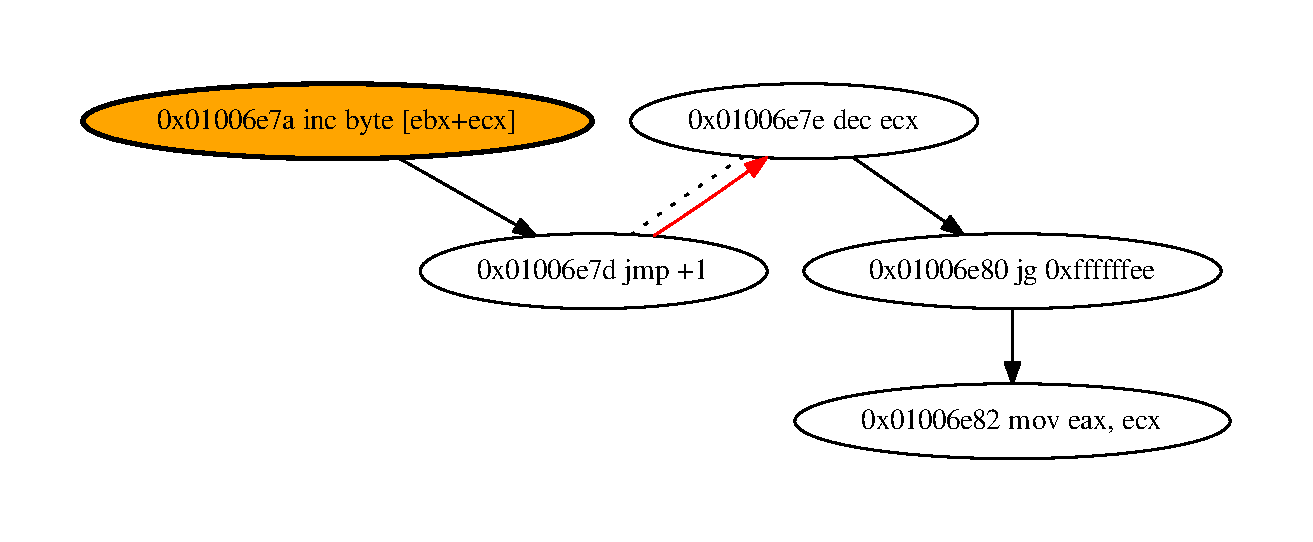
\includegraphics[width=0.8\textwidth]{supports/disasm/telock/telock.pdf}
\end{center}
\caption{Graphe de flot de contrôle de \telock}
\label{fig:telock_cfg}
\end{figure}

\paragraph{Exemple dans UPX.}

\section{Auto-modification}

% \begin{figure}
% \begin{center}
% \begin{tabular}{|l|l|l|}
% \hline
% Adresse & Octets & Instruction\\
% \hline
%  8048060  &  (...)         	& Pile -> RWX \\ 
%  804807c  &  bf 00 00 00 00         &  mov    edi, 0x0 \\
%  8048081  &  b8 91 80 04 08         &  mov    eax, 0x8048091 \\
%  8048086  &  66 c7 00 eb 00         &  mov    [eax], 0xeb \\
%  804808b  &  66 c7 40 01 07 00      &  mov    [eax+1], 0x7 \\
%  8048091  &  eb 0e                  &  jmp    80480a1 <edi3> \\
%  8048093  &  bf 01 00 00 00         &  mov    edi,0x1 \\
%  8048098  &  eb 0e                  &  jmp    80480a8 <fin> \\
%  804809a  &  bf 02 00 00 00         &  mov    edi,0x2 \\
%  804809f  &  eb 07                  &  jmp    80480a8 <fin> \\
%  80480a1  &  bf 03 00 00 00         &  mov    edi,0x3 \\
%  80480a6  &  eb 00                  &  jmp    80480a8 <fin> \\
%  80480a8  &  (...)		    &  Affiche edi \\
%  80480c3  &  (...)		    & Quitte \\
% \hline
% \end{tabular}
% \end{center}
% \caption{Exemple de code auto-modifiant}
% \label{fig:unevague_v0_code}
% \end{figure}

\begin{figure}
\begin{center}
\subfigure[Code assembleur]{
\begin{tabular}[b]{|l|l|l|}
\hline
Adresse & Octets & Instruction\\ 
\hline
 8048060  &  (...)         	& Pile -> RWX \\ 
 804807c  &  bf 00 00 00 00         &  mov    edi, 0x0 \\
 8048081  &  b8 91 80 04 08         &  mov    eax, 0x8048091 \\
 8048086  &  66 c7 00 eb 00         &  mov    [eax], 0xeb \\
 804808b  &  66 c7 40 01 07 00      &  mov    [eax+1], 0x7 \\
 8048091  &  eb 0e                  &  jmp    80480a1 <edi3> \\
 8048093  &  bf 01 00 00 00         &  mov    edi,0x1 \\
 8048098  &  eb 0e                  &  jmp    80480a8 <fin> \\
 804809a  &  bf 02 00 00 00         &  mov    edi,0x2 \\
 804809f  &  eb 07                  &  jmp    80480a8 <fin> \\
 80480a1  &  bf 03 00 00 00         &  mov    edi,0x3 \\
 80480a6  &  eb 00                  &  jmp    80480a8 <fin> \\
 80480a8  &  (...)		    &  Affiche edi \\
 80480c3  &  (...)		    & Quitte \\
\hline
\end{tabular}
\label{fig:unevague_v0_code}
}
\subfigure[Graphe de flot de contrôle]{
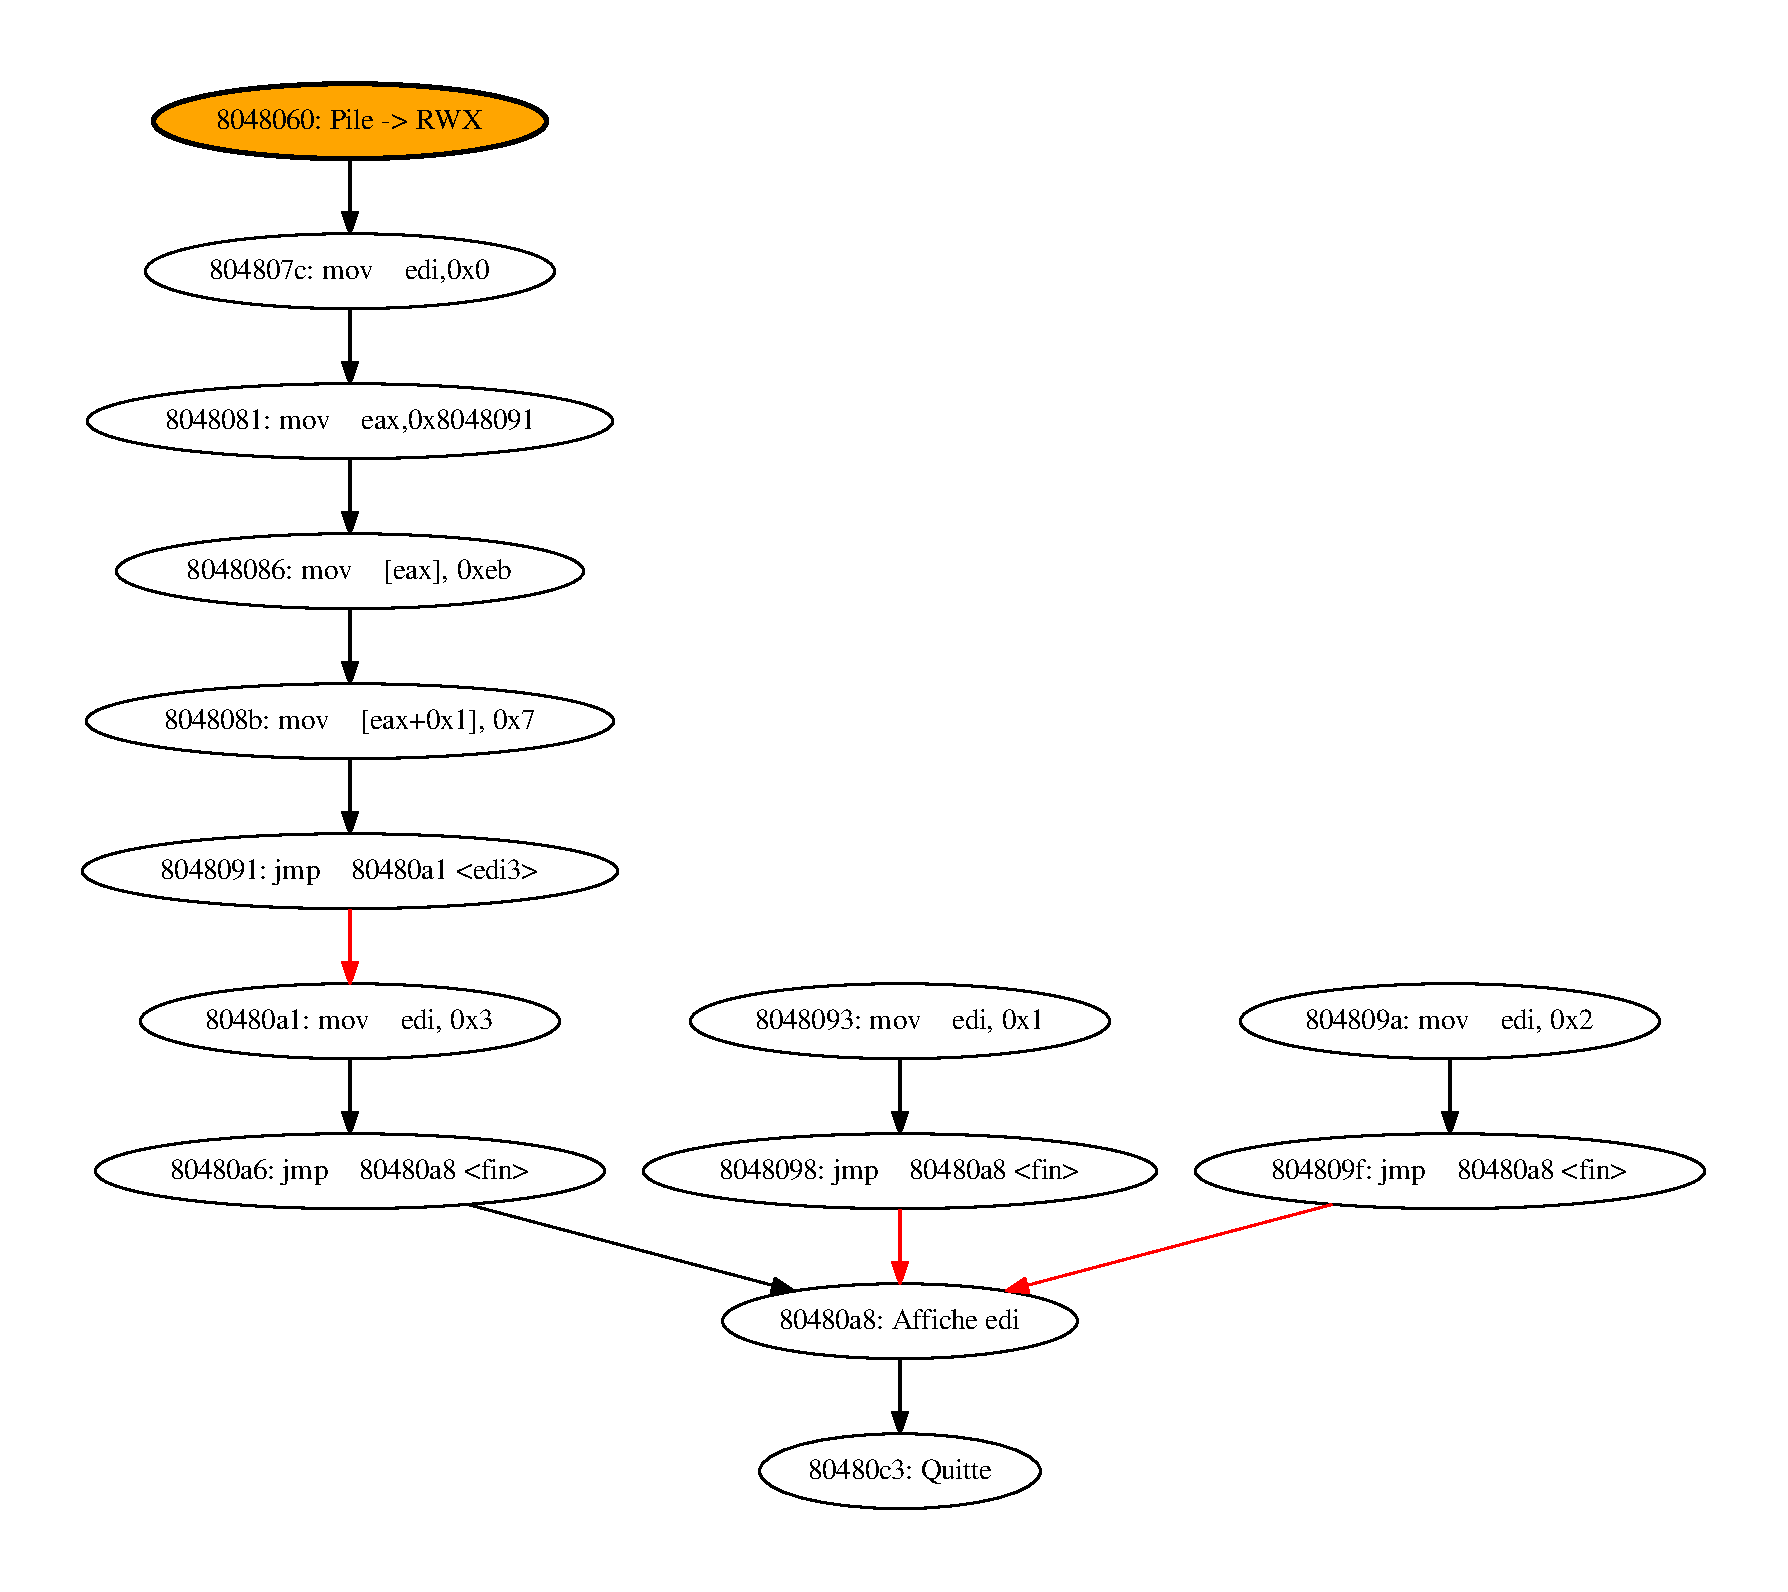
\includegraphics[width=1.0\textwidth]{supports/unevague/uv.pdf}
\label{fig:unevague_v0_cfg}
}
\end{center}
\ijym{détailler les ... (en annexe?)}
\ijym{fonction f, adresses f, f+1, f+3, ...}
\caption{Code assembleur auto-modifiant}
\label{fig:unevague_v0}
\end{figure}

Il a été expliqué dans la section \ref{section:assembleur} que, avec l'architecture de Harvard modifiée, le code n'est pas physiquement séparé des données lors de l'exécution sur une machine réelle.
Un programme auto-modifiant est simplement un programme utilisant cette propriété pour modifier le code assembleur le définissant au cours même de son exécution.
Ainsi on parle de comportement auto-modifiant lorsqu'une instruction du programme est codée sur au moins un octet qui a au préalable été modifié par ce programme.

En pratique les processeurs récents implémentent une protection, appelée bit NX ou W\textasciicircum X (prononcé ``W xor X''), permettant d'empêcher qu'une page mémoire puisse être à la fois écrite et exécutée lors de l'exécution du programme.
Cette protection a été ajoutée pour éviter des attaques résultant en l'exécution de code dans des données écrites par l'utilisateur du programme et non pour interdire l'auto-modification qui a des cas d'utilisation légitimes.
De ce fait l'activation ou non de la protection est spécifiée lors de la compilation et si un programme n'est pas protégé il lui suffit d'utiliser un appel système (\texttt{mprotect} sous linux) pour autoriser l'exécution de code sur la pile.

Prenons le programme de la figure \ref{fig:unevague_v0_code}. Ce programme commence par autoriser l'accès en écriture à la la section de code \ptext\ puis écrit sur la pile, modifie la valeur du registre \edi\ et termine par l'affichage de la valeur de \edi.
Si on ne prend pas en compte l'écriture sur la pile, il semble évident au vu du graphe de flot de contrôle (Figure \ref{fig:unevague_v0_cfg}), vu que la première instruction de saut provoque un saut vers l'instruction \texttt{mov edi,0x3} et que la seconde provoque l'affichage de \edi, que la valeur finale du registre est 3.
Pourtant les instructions \texttt{mov [eax],0xeb} et \texttt{mov [eax+1],0x07} aux l'adresse $0x8048086$ et $0x804808b$ remplacent le saut initial par un saut vers l'adresse $0x8048098$ où la valeur de \edi\ sera fixée à 2 avant l'affichage de celle-ci.


On constate ici que le programme se modifie au cours de son exécution et donc
\begin{itemize}
 \item On ne peut pas se contenter de la représentation d'origine du programme pour l'analyser.
 \item Le graphe de flot de contrôle initial peut être amené à évoluer au cours de l'exécution du programme.
\end{itemize}

\section{Logiciels malveillants et obscurcissement}
\itodo{packers, comment chaîner les obfuscations}
\itodo{utiliser des petites variations d'un packer pour éviter la détection, parler de la détection}

\section{Conclusion}
Cette thèse s'intéresse particulièrement à l'analyse des programmes écrits en assembleur \xq\ et \xs. Ces programmes ont en général été compilés à partir d'un langage de haut niveau puis ont été modifiés à l'aide d'un logiciel de protection. Les binaires que l'on étudie sont donc protégés avec des techniques statiques comme auto-modifiantes. Notre travail consiste alors à chercher à désassembler correctement ces programmes dans le but de faciliter leur analyse.

Les chapitres suivants détailleront plusieurs techniques d'analyse que nous avons appliquées. Nous nous intéresserons d'abord à l'aspect auto-modifiant des programmes et verrons comment l'analyse dynamique peut être utilisée pour reconstruire un modèle pour le programme auto-modifiant. Dans un second temps nous introduiront des techniques d'analyse statiques pour chercher à recomposer le maximum de code assembleur du programme et contourner d'autres méthodes de protection comme le chevauchement de code.

% \DontFrameThisInToc

\chapter{Application à la détection de similarités logicielles\label{chap:libs}}
L'analyse morphologique appliquées aux graphes de flot de contrôle de plusieurs binaires peut également être utilisée pour détecter l'utilisation de fonctionnalités similaires entre ces programmes et faire correspondre précisément des morceaux de code assembleur de l'un et de l'autre.

Dans ce chapitre nous présentons des travaux réalisés en ce sens sur un logiciel malveillant, Waledac, qui utilise une bibliothèque connue de chiffrement, OpenSSL.
Ces travaux ont fait l'objet d'une communication orale à REcon en 2012 \cite{REAT12} et d'une publication à Malware \cite{mal12}.

% \section{Problème : accélérer l'analyse}
\section{Contexte d'analyse de code}
L'analyse manuelle de codes binaires inconnus est à la base de tout travail sur la détection de logiciels malveillants.
L'analyste cherche d'une part à déterminer et comprendre l'ensemble du code du programme afin d'en connaître les fonctionnalités
et le classer comme logiciel malveillant ou légitime.
D'autre part, s'il s'agit d'un logiciel malveillant, il cherche à établir une signature du binaire permettant de détecter sa présence sur une machine infectée et éventuellement de le supprimer.
L'analyse se fait à l'aide de différents outils, dont un désassembleur interactif tel IDA \cite{IDA} ou Radare \cite{radare} pour l'analyse statique et d'un outil pour l'analyse dynamique comme un débogueur, un émulateur ou un logiciel d'instrumentation.

Les logiciels analysés ne présentent en général pas d'informations de compilation permettant d'identifier les bibliothèques logicielles utilisées ni leur version. Nous cherchons à automatiser la recherche de bibliothèques connues dans un logiciel à analyser et à marquer son emplacement dans un désassembleur interactif (IDA) afin d'éviter l'analyse inutile de code documenté et d'accélérer l'analyse manuelle.

\subsection{Waledac et OpenSSL}
Waledac \cite{CRFLSGBA10}, apparu en 2008, est un botnet, c'est à dire un programme malveillant transformant les machines infectées en esclaves (ou \emph{zombies}) recevant des ordres d'un serveur de commande et de contrôle (C\&C).
Les machines esclaves communiquent entre elles sous la forme d'un réseau pair à pair et la charge finale principale du réseau est l'envoi de courrier électronique non sollicité (\emph{spam}).
Il s'agit d'un programme dont les fonctionnalités étaient déjà bien connues et documentées lorsque nous avons commencé à nous y intéresser. Notre objectif était alors de voir s'il était possible d'automatiser une partie de l'analyse, sachant que nous serions capables de vérifier nos résultats à l'aide d'analyses manuelles existantes.

Afin de savoir quelles méthodes de chiffrement le programme utilise, nous avons cherché des chaînes de caractères dans le binaire correspondant à quelques bibliothèques standard à l'aide du l'outil \emph{strings}.
Par chance il a été facile de trouver qu'il utilise la version 0.9.8e d'OpenSSL:
\begin{verbatim}
$ strings "Waledac v48 unpacked.exe" | grep OpenSSL
   EC part of OpenSSL 0.9.8e 23 Feb 2007
   ECDSA part of OpenSSL 0.9.8e 23 Feb 2007
\end{verbatim}

OpenSSL \cite{openssl} est une bibliothèque libre et documentée, elle ne devrait pas nécessiter une analyse de son code binaire ici inclus dans Waledac. Nous voulons aller plus loin afin de connaître précisément les fonctions utilisées ainsi que les parties de code communes.

\section{Analyse morphologique}
% \subsection{Trouver des sites communs}
La technique d'analyse morphologique détaillée aux deux chapitres précédents a été directement utilisée : on détermine les graphes de flot de contrôle de chacun des deux binaires, on leur applique des réductions puis on les découpe en sites.
On cherche ensuite des sites communs entre les Waledac et OpenSSL.

\paragraph{Taille des graphes de flot.}
Les binaires sur lesquels nous avons travaillé ont des graphes de flot de contrôle initiaux allant jusqu'à quelques centaines de milliers de sommets avant réduction et environ quinze mille sommets après réduction. Nous avons initialement trouvé 53 sites communs entre la version 0.9.8x d'OpenSSL et Waledac.
Nous avons initialement pris la version 0.9.8x, la version à jour d'OpenSSL, parce que les versions antérieures n'étaient pas disponibles sous forme binaire pour Windows et nécessitaient d'être compilées.

\begin{figure}[h]
\begin{center}
\begin{tabular}{|l|r|r|r|}
\hline
 Binaire & Taille du GFC & Taille du GFC réduit & Nombre de sites de taille 24 	\\
\hline
 Waledac &  38236 & 14626 & 11141					  	\\
\hline
 OpenSSL 0.9.8x  & 174754 & 28313 & 22171				  	\\
\hline
\end{tabular}
\end{center}
\end{figure}

\paragraph{Influence des options de compilation.}
Nous avons ensuite compilé la version 0.9.8e en utilisant différentes options de compilation utilisées avec le compilateur pour Windows Visual Studio.
Nous avons pu remarquer que l'option donnant le plus sites en commun était celle compilée pour optimiser la taille du binaire. Le tableau suivant donne le nombre de sous-sites communs entre Waledac et chacune des versions d'OpenSSL.

\begin{figure}[h]
\begin{center}
\begin{tabular}{|l|l|r|}
 \hline
Version & Remarque & Sites communs \\
 \hline
0.9.8x & Version de mai 2012 & 53 \\
0.9.8e & Optimise les performances temporelles (/0x /02) & 53 \\
0.9.8e & Optimise la taille du fichier (/01) & 1264 \\
 \hline
\end{tabular}
\end{center}
\end{figure}

\subsection{Correspondance fine entre instructions}
Dans un second temps nous avons voulu être capables de marquer, dans le désassembleur interactif utilisé, les instructions ainsi que les fonctions assembleur qui ont été reconnues.
Nous avons utilisé les techniques précédentes pour qu'en plus de retourner une correspondance entre un site du graphe de motif P et un site du graphe de test T, nous ayons aussi l'information précise donnant la correspondance entre un sommet du sous-site de motif et un sommet du sous-site de test. Tous les algorithmes présentés au chapitre précédent peuvent fournir cette information.

Nous supposons donc que l'on dispose de la fonction \emph{match} qui, à partir d'un sous-site $S_P$ de $P$ et d'un sous-site $S_T$ de $T$, renvoie une liste de couples de correspondance entre un sommet de $S_P$ et un sommet de $S_T$. Dans le cas où les deux sous-sites ne correspondent pas, elle renvoie $\emptyset$.

Comme décrit dans l'algorithme \ref{algo:correspondance_fine}, nous considérons que plus la taille des sous-sites correspondants est grande, plus la correspondance entre les sommets sera précise.
Nous cherchons en premier lieu le plus grand sous-site que l'on retrouve dans P et T et nous associons tous les sommets de P et de T  correspondants dans ce sous-site. Nous récupérons l'ensemble des sous-sites d'une certaine taille de $P$ et $T$ à l'aide de l'algorithme \ref{algo:generation_site_largeur} du chapitre précédent.
Puis nous continuons avec un sous-site commun plus petit, en associant les sommets qui n'ont pas encore été associés, et ainsi de suite jusqu'à atteindre la taille initiale des sites choisis pour la détection, soit W. 

\begin{figure}[h]
\begin{algorithm}[H]
\DontPrintSemicolon
\caption{Association des sommets de deux graphes de flot de contrôle}
\SetAlgoLined
\KwIn{Deux graphes de flot, P et T de taille respective $n_P$ et $n_T$, la taille minimale des sites recherchés, W}
\KwResult{Une liste de correspondances sommet à sommet entre P et T}
\SetKwProg{Fn}{}{}{}
\SetKwFunction{FRecurs}{association}
\Fn(
% \tcc*[h]{C : matrice des associations possibles, i : numéro du prochain sommet de P à associer, F : liste des couples d'associations déjà faites}
){\FRecurs{P, $n_P$, T, $n_T$, W}}{
$L\leftarrow \emptyset$\\
$A_P, A_T \leftarrow (\emptyset, \emptyset)$ \tcc*{ensembles des sites de T et P associés}
$m\leftarrow min(n_P, n_T)$\\
\tcc{On extrait tous les sites :}
\For {$W \leq i\leq m$} {
  $S_{P, i}\leftarrow sites(P, i)$\\
  $S_{T, i}\leftarrow sites(T, i)$
}
$k\leftarrow m$\\
\While{$k\geq W$}{
\For{$S_P\in S_{P, k}$}
{
  \For{$S_T\in S_{T, k}$}
  {
    \tcc{On place dans C les couples de sommets correspondants :}
    $C\leftarrow match(S_P, S_T)$ 
    \For{$(s_P, s_T)\in C$}{
      \If{$s_P\notin A_P$ et $s_T\notin A_T$}{
	$L\leftarrow L\cup \{(s_P, s_T)\}$\\
	$A_P\leftarrow A_P\cup \{s_P\}$\\
	$A_T\leftarrow A_T\cup \{s_T\}$\\
      }
    }
  }
}
$k\leftarrow k-1$
}
\Return{L}
}
\label{algo:correspondance_fine}
\end{algorithm}
\end{figure}

\subsection{Implémentation et résultats}
\paragraph{Correspondance entre sommets.}
La fonction \emph{match} donnant les correspondances a été implémentée pour une variante de l'algorithme d'Ullmann présentée au chapitre précédent, variante adaptée à la comparaison de sites de même taille.
Elle a également été implémentée dans la version d'origine du détecteur fonctionnant par automates d'arbres.
Nous avons ajouté dans le détecteur une possibilité d'export de ces correspondances.

\paragraph{Greffon IDA.}
Un greffon (ou \emph{plugin}) a été développé pour le désassembleur interactif IDA, permettant, lorsque que deux instances du désassembleur sont lancées, chacune analysant un des deux programmes comparés, d'aligner le code comparé selon les correspondances trouvées au préalable par analyse morphologique.
Le greffon surligne les instructions ayant trouvé un correspondant dans l'autre graphe de flot et donne également la correspondance entre les fonctions assembleur du premier programme et du second.

\paragraph{Exemple avec Waledac et OpenSSL.}
La figure \ref{fig:plugin_subroutines} montre un extrait de la page de correspondances entre les fonctions assembleur identifiées par IDA entre la DLL principale d'OpenSSL (\emph{libeay32-098e.dll}) et Waledac (\emph{Waledac48.int}). La première colonne indique les adresses des instructions d'OpenSSL correspondant aux instructions présentes aux adresses de Waledac situées à la troisième colonne. Les deuxième et quatrième colonnes donnent le nom des fonctions assembleur auxquelles ces instructions appartiennent.
OpenSSL ayant été compilé avec des options de débogage, le nom des fonctions est retrouvé par IDA, ce qui n'est pas le cas pour Waledac.
Il est à noter que, puisqu'on a effectué des réductions avant de lancer la comparaison, la plupart des instructions, dont les instructions séquentielles, ne sont pas comparées : ce sont principalement les instructions modifiant le flot de contrôle qui ont été considérées.

% \begin{figure}[h]
% \begin{center}
%  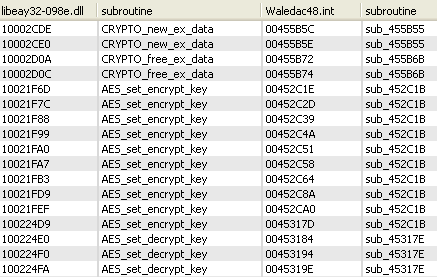
\includegraphics[width=0.8\textwidth]{supports/libs/WalSSLIDA2.png}
% \end{center}
% \caption{Fonctions correspondantes entre OpenSSL à gauche et Waledac à droite}
% \label{fig:plugin_subroutines}
% \end{figure}

\begin{figure}[h]
\begin{center}
\begin{tabular}{|l|l|l|l|}
\hline
\multicolumn{2}{|c|}{OpenSSL (libeay32-098e.dll)} & \multicolumn{2}{c|}{Waledac (Waledac48.int)} \\
\hline
Adresse & Fonction & Adresse & Fonction \\
\hline
 10002CDE & CRYPTO\_new\_ex\_data & 00455B5C & sub\_455B55 \\
 10002CD0 & CRYPTO\_new\_ex\_data & 00455B5E & sub\_455B55 \\
 10002D0A & CRYPTO\_new\_ex\_data & 00455B72 & sub\_455B55 \\
 10002D0C & CRYPTO\_new\_ex\_data & 00455B74 & sub\_455B55 \\
\hline
 10021F6D & AES\_set\_encrypt\_key & 00452C1E & sub\_452C1B \\
 10021F7C & AES\_set\_encrypt\_key & 00452C2D & sub\_452C1B \\
 10021F88 & AES\_set\_encrypt\_key & 00452C39 & sub\_452C1B \\
 10021F99 & AES\_set\_encrypt\_key & 00452C4A & sub\_452C1B \\
 10021FA0 & AES\_set\_encrypt\_key & 00452C51 & sub\_452C1B \\
 10021FA7 & AES\_set\_encrypt\_key & 00452C58 & sub\_452C1B \\
 10021FB3 & AES\_set\_encrypt\_key & 00452C64 & sub\_452C1B \\
 10021FD9 & AES\_set\_encrypt\_key & 00452C8A & sub\_452C1B \\
 10021FEF & AES\_set\_encrypt\_key & 00452CA0 & sub\_452C1B \\
 100224D9 & AES\_set\_encrypt\_key & 0045317D & sub\_452C1B \\
\hline
 100224E0 & AES\_set\_decrypt\_key & 00453184 & sub\_45317E \\
 100224F0 & AES\_set\_decrypt\_key & 00453194 & sub\_45317E \\
 100224FA & AES\_set\_decrypt\_key & 0045319E & sub\_45317E \\
\hline
\end{tabular}
\end{center}
\caption{Fonctions correspondantes entre OpenSSL et Waledac}
\label{fig:plugin_subroutines}
\end{figure}


Nous avons ensuite vérifié dans IDA, grâce à la fonction d'alignement de code du greffon, que le code des instructions correspondantes était bien suffisamment similaire pour valider la méthode.
Une telle correspondance est donnée en exemple à la figure \ref{fig:plugin_code_sync} pour la fonction \emph{AES\_set\_encrypt\_key}.
L'image est constituée d'un bout du graphe de flot de contrôle d'OpenSSL à gauche et d'un bout du GFC de Waledac à droite.
Les instructions surlignées en orange et alignées sont celles pour lesquelles on a trouvé une correspondance.

\begin{figure}[h]
\begin{center}
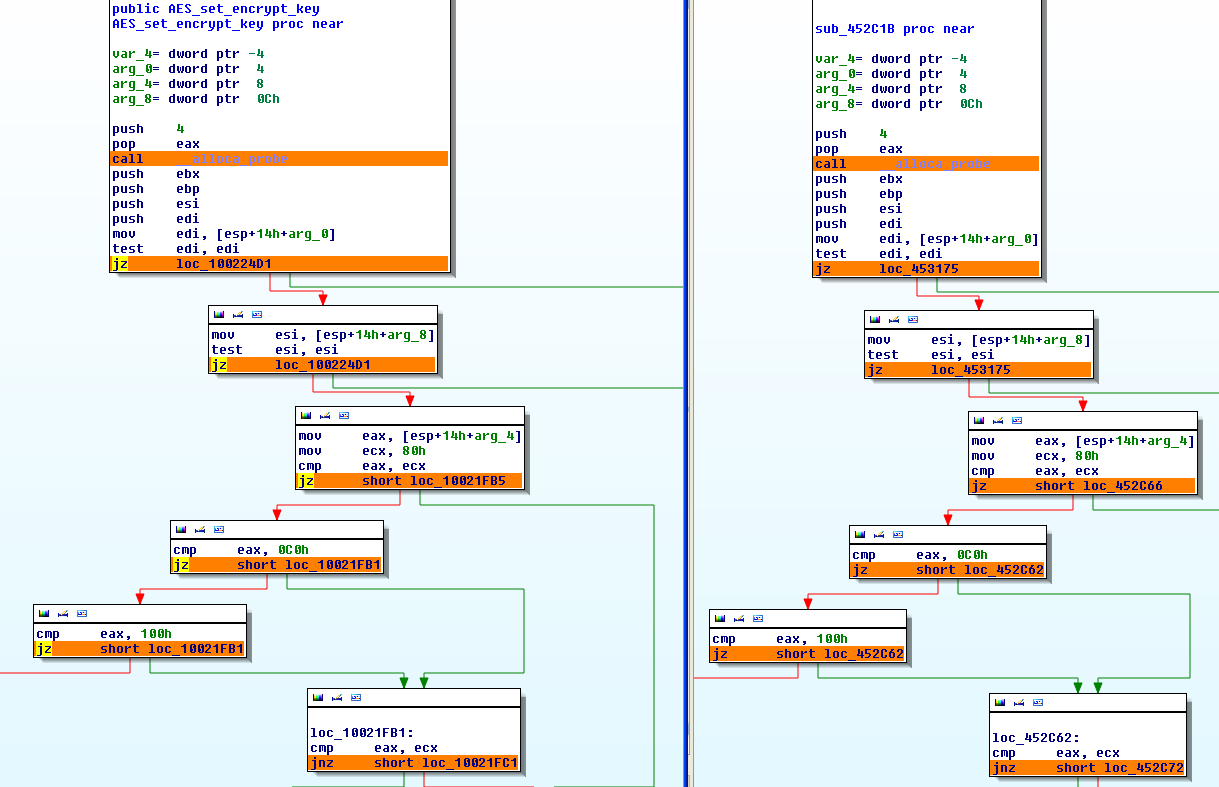
\includegraphics[width=1.0\textwidth]{supports/libs/WalSSLIDAAESgraph.png}
\caption{Capture d'écran d'IDA : Code correspondant entre OpenSSL à gauche et Waledac à droite} 
\label{fig:plugin_code_sync}
\end{center}
\end{figure}

Sur cet exemple nous n'avons pas trouvé de correspondance sommet à sommet qui ne soit pas cohérente mais certaines fonctions n'étaient pas couvertes par suffisamment de sommets pour que l'on soit assuré d'une correspondance.
La figure \ref{fig:tab_fonctionnalites_waledac_openssl} donne un extrait des fonctions d'OpenSSL retrouvées dans Waledac et les fonctionnalités qu'elles fournissent : on y trouve par exemple des méthodes préparant au chiffrement AES, RSA et DSA.

\begin{figure}[h]
\begin{tabular}{|p{9cm}|l|}
\hline
Fonctions 							& Fonctionnalité 			\\
\hline
AES\_set\_encrypt\_key, AES\_set\_decrypt\_key 			& Chiffrement AES 			\\
RSA\_free, DSA\_size, DSA\_new\_method 				& Chiffrement RSA / DSA 		\\
 X509\_PUBKEY\_set, X509\_PUBKEY\_get 				& Certificats X509 			\\
BN\_is\_prime\_fasttest\_ex, BN\_ctx\_new, BN\_mod\_inverse	& Gestion des grands entiers (BN)	\\
CRYPTO\_lock, CRYPTO\_malloc 					& Fonctions génériques d'OpenSSL 	\\
\hline
\end{tabular}
\caption{Fonctions d'OpenSSL retrouvées dans Waledac et fonctionnalités associées}
\label{fig:tab_fonctionnalites_waledac_openssl}
\end{figure}

Il n'est pas surprenant que l'on retrouve ces fonctionnalités puisque Waledac utilise du chiffrement AES et RSA et gère des certificats X509. Notre contribution est l'emploi de la technique d'analyse morphologique pour déterminer automatiquement ces informations sans analyser manuellement le code assembleur.

\section{Limites}
On a vu qu'on retrouve certaines fonctions utilisées lors d'un chiffrement AES.
Pourtant nous n'avons pas retrouvé les fonctions principales servant à chiffrer et déchiffrer à l'aide de l'algorithme AES.
La raison est que notre approche par graphes de flot réduits s'applique très mal aux fonctions de chiffrement qui sont en général très simples du point de vue de leur graphe de flot de contrôle.
Une vue simplifiée du GFC de la fonction \emph{AES\_encrypt} est donnée en figure \ref{fig:AES_encrypt_CFG}.

\begin{figure}[h]
\begin{center}
% \subfigure[AES\_encrypt subroutine]{
% 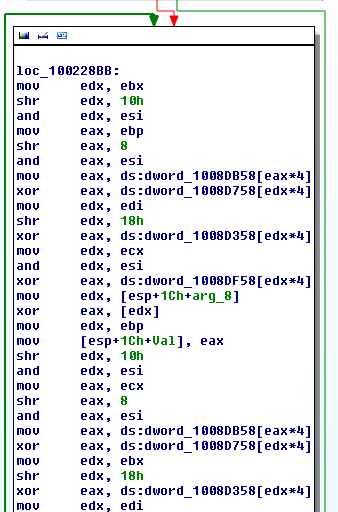
\includegraphics[width=0.4\textwidth]{supports/libs/WalSSLIDAAESencryptnotmatched.png}
% \label{fig:AES_encrypt_IDA}
% }
% \subfigure[]{
\includegraphics[width=0.25\textwidth]{supports/libs/AESsimpleCFG_cropped0.pdf}

% }
\end{center}
\caption{GFC simplifié de la fonction AES\_encrypt}
\label{fig:AES_encrypt_CFG}
\end{figure}

Le GFC réduit est trop petit pour pouvoir être détecté par l'analyse morphologique qui prend des graphes d'une taille 24 au minimum.
En fait beaucoup d'algorithmes de chiffrement ont cette structure une fois réduits et elle n'est pas non plus spécifique aux algorithmes de chiffrement. De ce fait l'analyse morphologique est inadaptée à la détection de ce genre de fonctions.

\section{Application à Duqu et Stuxnet}
Dans cette section nous présentons nos travaux sur deux programmes malveillants particuliers, \duqu\ et \stux.
Lorsque nous avons commencé ces travaux \stux\ était déjà documenté et détecté et \duqu\ venait d'être découvert.
Il a rapidement été dit qu'ils étaient semblables et nous avons donc cherché à détecter \duqu\ connaissant \stux.
% Dans un premier temps nous appliquons les travaux présentés au chapitre précédent sur ces exemples \cite{REAT12,mal12}.

\subsection{Duqu et Stuxnet}
% \paragraph{\stux.}
\stux, découvert en juin 2010, est capable de cibler et de reprogrammer des systèmes industriels.
Sans que cela ait été prouvé, il a été avancé qu'il visait le programme nucléaire iranien. 
Symantec \cite{SymantecStux2011} indique que la plupart des systèmes infectés sont en Iran et que la cible pourrait être un système de contrôle de centrifugeuses.
\\

% \paragraph{\duqu.}
\duqu, découvert en premier par Crysys \cite{CrysysDuquStuxnet} en septembre 2011, laboratoire de sécurité et de cryptographie de l'université de Budapest, a directement été détecté comme apparenté à \stux\ parce que ces deux programmes utilisent des techniques d'infection et de propagation similaires.
\duqu\ est un outil offensif utilisé pour le vol d'informations. Symantec \cite{SymantecDuqu2011} a identifié parmi ses fonctionnalités des enregistreurs de frappes (\emph{keyloggers}), de l'écran, de l'activité réseau ainsi que des outils de détection de machines sur le réseau.
Il est maintenu à jour via des serveurs de commande et de contrôle (C\&C) et dispose d'une fonctionnalité d'auto-destruction après, typiquement, 36 jours sans nouvelles du C\&C.

Les attaques semblent réussies puisque le programme malveillant n'a pas été détecté à chaud alors que certaines opérations ont duré plusieurs mois, mais seulement post-mortem. De nombreuses souches de \duqu\ ont été trouvées dans la natures, chacune avec des binaires différents mais similaires. Kaspersky a publié un historique des versions \cite{KaspDuqu10}, la dernière souche détectée date de février 2012, bien après que les première attaques n'ont été détectées et documentées.

\paragraph{Analyse des similarités.}
Nous avons effectué une analyse similaire à celle décrite au chapitre précédent pour trouver les similarités entre \stux\ et \duqu\ afin de trouver les parties de \stux\ que l'on retrouve dans \duqu.
Pour ces deux programmes malveillants, nous avons analysé la DLL (bibliothèque logicielle au format Windows, ou \emph{Dynamic Link Library}) principale une fois que celle-ci a été déchiffrée.
% Dans les deux cas l'infection est cherche à exploiter une faille de Windows permettant d'installer plusieurs composants qui auront été déchiffrés au préalable.
Nous avons extrait les graphes de flot réduits de \duqu\ et \stux.
Nous avons trouvé 846 sites communs entre \duqu\ et \stux\ : 26.5\% des sites de \duqu\ proviennent de \stux.
Lorsque l'on regarde les sommets correspondants dans les graphes réduits, on s'aperçoit que ces sites contiennent 2215 sommets dans les graphes de flot réduits : 60.3\% des sommets du graphe de flot réduit de \duqu\ correspondent à des sommets  présents dans \stux.

Forts de ces résultats indiquant que \duqu\ et \stux\ partagent beaucoup de code, nous considérons donc qu'un détecteur de programmes malveillants fonctionnant avec la technique d'analyse morphologique connaissant \stux\ serait capable de détecter \duqu.

La principale difficulté que doit résoudre un détecteur est que le programme provocant l'infection de \duqu\ ne ressemble pas à \stux\ ni à aucun autre programme malveillant connu. Ce n'est que lorsque certains composants de \duqu\ sont déchiffrés et installés que l'on peut le détecter.
Nous détaillons dans le chapitre suivant la méthode d'infection de \duqu\ et le travail nécessaire afin de détecter une attaque.
% Nous avons alors cherché à documenter la méthode d'infection de \duqu\ afin de pouvoir détecter une attaque.


\section{Perspectives}
Un approfondissement de cette approche à l'analyse de similarités logicielles serait intéressant. D'une part nous voudrions effectuer des expériences sur plus d'échantillons de code malveillant pour confirmer les résultats prometteurs mis en lumière dans ce chapitre.
D'autre part nous souhaiterions comparer en détail notre approche à celles existantes, notamment par rapport à une comparaison directe des instructions des binaires.

\section*{Conclusion}
Nous avons identifié des similarités entre Waledac et une version spécifique d'OpenSSL, nous avons pu reconstruire automatiquement des correspondances fines afin de déterminer quelles fonctions d'OpenSSL ont été utilisées par Waledac.
L'obstacle principal à une généralisation de cette méthode est qu'elle est sensible aux options de compilation et nécessite de déterminer au préalable les binaires à comparer.
Cette technique n'est pas infaillible puisqu'elle n'est pas adaptée pour détecter certaines structures ou fonctions, telles des fonctions de chiffrement.

Nous avons ensuite développé un greffon pour IDA permettant d'analyser les similarités trouvées afin de permettre à l'analyste de ne pas s'attarder sur du code déjà documenté.
Cette approche, appliquée à \duqu\ et \stux\ nous a permis de mettre en lumière de nombreuses portions de code partagées entre ces deux logiciels malveillants.

\chapter{Cas d'étude : Duqu et Stuxnet\label{chap:duqu-stux}}
Dans ce chapitre nous continuons nos travaux sur deux programmes malveillants particuliers, \duqu\ et \stux, dont nous avons montré qu'ils partageaient du code au chapitre précédent.
Notre objectif est de pouvoir détecter une attaque par \duqu\ connaissant \stux.
% cela nécessite un accès au code déchiffré et injecté par \duqu.

Nous cherchons donc à détecter \duqu\ avant qu'il ne puisse infecter une machine ciblée.
Nous étudions pour cela un composant spécifique de \duqu, son pilote (\emph{driver}) qui permet de charger discrètement le code malveillant en mémoire.
Notre contribution consiste en la rétroingénierie de ce composant, en la reconstitution de son code source et en une analyse de son fonctionnement.
Nous avons détournons ensuite le pilote pour en faire une version défensive capable de détecter d'éventuelles attaques similaires.
En particulier nous montrons comment le pilote de \duqu\ modifié permet de détecter et d'empêcher une attaque par \duqu.
Ces travaux ont fait l'objet d'une publication à SSTIC \cite{sstic13} ainsi qu'à  Malware \cite{mal13}.

\section{Détection d'une infection par Duqu}
\subsection{Déroulement d'une infection}
L'infection détectée par Crysys utilise un document Microsoft Word piégé, incluant \duqu.
Dans un premier temps il exploite une faille jusque là inconnue (\emph{0-day} sur les polices d'écriture TrueType \cite{CVETrueType}) du noyau Windows afin d'installer trois composants sur le système :
\begin{itemize}
 \item Un pilote : \driver
 \item Une DLL chiffrée : \netpDLL
 \item Un fichier de configuration chiffré : \netpCONF
\end{itemize}

Au redémarrage de la machine, le pilote surveille le chargement des processus par le système d'exploitation et injecte la DLL principale de \duqu, une fois déchiffrée, dans un processus spécifié par le fichier de configuration, typiquement \services.
Enfin le pilote modifie \services\ afin qu'il exécute la charge finale, qui est incluse dans la DLL.

Une fois installé sur une première cible \duqu\ reçoit des ordres d'attaque et de propagation d'un serveur C\&C.
Chaque machine infectée peut être configurée pour se connecter à l'attaquant, pas directement mais par la machine qui l'a infectée, créant une sorte de tunnel de routage pour des machines non accessibles directement depuis l'extérieur. Une illustration de ce mécanisme est donnée en figure \ref{fig:propagationDuqu}.

\begin{figure}[h]
\begin{center}
 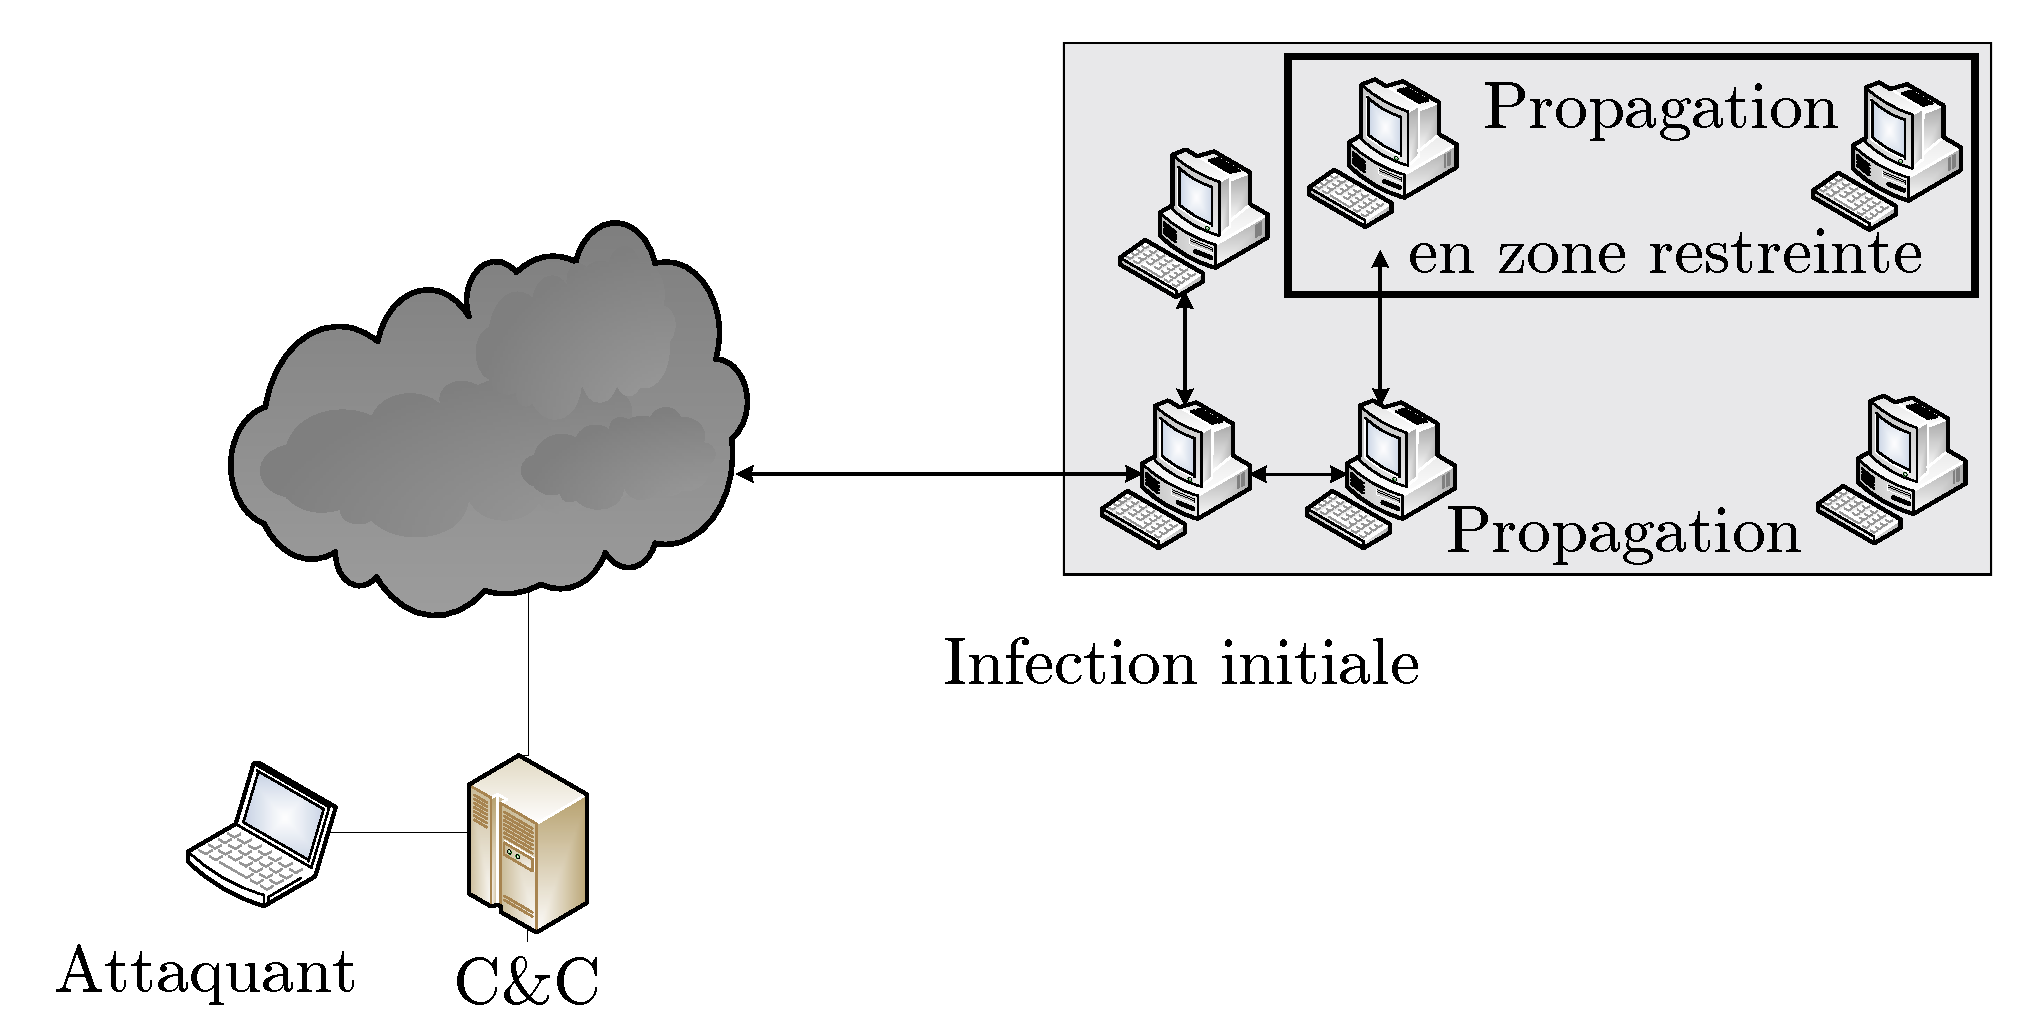
\includegraphics[width=0.8\textwidth]{supports/duqu/propagationDuqu2.pdf}
 % graph11.eps: 0x0 pixel, 300dpi, 0.00x0.00 cm, bb=0 0 384 336
\end{center}
\caption{Schéma de propagation en profondeur de Duqu}
\label{fig:propagationDuqu}
\end{figure}

\paragraph{Difficulté de la détection.}
L'obstacle principal à la détection est que seul le pilote est présent déchiffré sur le disque.
La DLL est chiffrée et empaquetée avec UPX, elle n'apparaît déchiffrée qu'en mémoire, lorsqu'elle est injectée dans \services.

\paragraph{Angle d'attaque pour une détection.}
L'attaque peut être détectée au moment du déchiffrement de la DLL principale et de son injection.
Elle doit prendre place après le déchiffrement mais avant que la charge finale ne soit exécutée.
Nous aurons pour cela besoin de suivre les processus lancés et de pouvoir analyser les DLL qu'ils exécutent.
Étant donné que le pilote de \duqu\ réalise cette opération, nous avons choisi de le modifier de telle sorte qu'il puisse s'interfacer avec le détecteur par analyse morphologique.
Pour mettre ce plan en \oe uvre, nous avons
\begin{itemize}
 \item reconstitué, par rétroingénierie, le code source du pilote de \duqu\ à partir de son binaire.
 \item modifié son code pour qu'il surveille le chargement des processus sans provoquer d'injection.
%  \item Interfacé le nouveau pilote avec notre outil de détection.
\end{itemize}

\subsection{Reconstruction du code du pilote}
Nous savions donc que les DLL principales de \duqu\ et \stux\ partageaient du code.
Le pilote de \stux\ a été décompilé par Amr Thabet \cite{ThabetDriver}.
Nous avons voulu suivre la même route et désassembler le pilote de \duqu\ afin de le documenter.
Nous avons eu à notre disposition la souche du pilote découverte en octobre 2011 en Europe : \driver.

Nous avons donc travaillé sur la rétroingénierie de cette version spécifique du pilote afin d’en documenter les fonctionnalités. 
Notre objectif est d’obtenir un code compréhensible que l'on peut compiler et dont la version compilée soit au plus proche du binaire d'origine.

\subsubsection{Décompilation avec IDA}
Nous avons utilisé le module de décompilation "Hex-Rays Decompiler", intégré à IDA sous la forme d’un greffon \cite{IDADecompiler}.
Il permet de générer un pseudo-code C à partir du fichier binaire en cours d’analyse.
Il produit non seulement du code source mais facilite également sa réécriture directement à l’intérieur de l’interface graphique du greffon. 
Malheureusement le code en sortie n’est, dans notre cas, pas exploitable directement. 
D’une part le code n’est pas compilable parce que des types de variables n’ont pas été correctement reconnus et certaines conventions d’appel ne sont pas standard (non reconnues par le décompilateur). 
De plus le code généré est difficilement lisible en partie parce que certaines structures n’ont pas été identifiées.
Nous détaillons dans les paragraphes suivants ces difficultés et des moyens de résolution.

Nous avons procédé de manière incrémentale afin de reconstruire le code petit à petit en vérifiant à chaque étape que le code compile et qu'une fois compilé il est équivalent à celui du binaire \driver\ original. 
Cela a consisté à :
\begin{itemize}
 \item commenter tout le pseudo-code sauf la fonction du point d'entrée du pilote (\emph{DriverEntry}) et les variables globales s'y rapportant,
 \item régler chaque erreur une par une,
 \item comparer le code compilé au binaire original, modifier le code pour s'en rapprocher,
 \item ajouter du code auparavant commenté et revenir à l'étape de correction d'erreurs.
\end{itemize}

\subsubsection{Identification des structures et des types}
La figure \ref{fig:ParsePEInitial} montre les premières lignes du code C reconstruit par le décompilateur pour une des fonctions du pilote.
Beaucoup d'informations manquent. Par exemple la plupart des types sont décrits comme des entiers (ou des pointeurs) : il n'est pas possible de savoir quel type de données cette fonction manipule.
Nous allons détailler sur cet exemple quelques techniques permettant de récupérer ces informations.

\begin{figure}[h]
\begin{center}
\begin{lstlisting}[language={C}]
signed int __cdecl sub_12F36(int a1, int a2, int a3)
{
  int v4; // eax@3
  unsigned __int16 v5; // cx@4
  int v6; // ecx@7

  v4 = a2 + *(_DWORD *)(a2 + 60);
  if (*(_DWORD *)v4 ^ 0xF750F284 != 0xF750B7D4)
    return 1;
\end{lstlisting}
\end{center}
\caption{Premières lignes de la fonction ParsePE décompilée par IDA\label{fig:ParsePEInitial}}
\end{figure}

Certaines constantes peuvent nous aider : par exemple \texttt{0xF750F284 XOR 0xF750B7D4 = 0x00004550} , qui représente la chaîne de caractères 'PE$\backslash$0$\backslash$0' en ASCII. Le texte est obscurci à l'aide d'une opération de ou exclusif (\emph{XOR}).

Nous soupçonnons alors que cette fonction est utilisée pour le traitement de fichiers binaires au format PE.
La documentation officielle de Microsoft Visual C++ détaille la structure PIMAGE\_NT\_HEADERS dont le premier champ, \emph{Signature}, vaut \PEzz\ pour les binaires Windows.
Ainsi la variable \texttt{v4}, qui est comparée à \PEzz, est probablement du type PIMAGE\_NT\_HEADERS.
Nous forçons ce type pour cette variable au sein d'IDA à la place du type \texttt{int} et IDA trouve automatiquement le nom des champs de ce type de variable à partir de leur décalage (\emph{offset}) en mémoire.
Lorsque les structures sont spécifiques au binaire analysé, il est possible de les définir manuellement dans le décompilateur.
Nous avons retrouvé les types des autres variables de manière similaire.

La figure \ref{fig:ParsePEFinal} donne les premières lignes de la fonction retouchée.
Elle est lisible par un développeur C : on peut voir que la fonction vérifie si un fichier est binaire PE.
Le reste de la fonction parcourt le binaire PE passé en entrée et remplit une structure spécifique avec quelques informations (son point d'entrée, ses sections, etc.).
De plus le code compilé de cette fonction est très similaire au binaire d'origine.


\begin{figure}[h]
\begin{center}
\begin{lstlisting}[language={C}]
NTSTATUS __cdecl ParsePE(__out PEDataPtr pPEData, 
    __in PIMAGE_DOS_HEADER BaseAddress, __in int flag){
PVOID infosPE;
PIMAGE_DOS_HEADER pDosHeader;
PIMAGE_NT_HEADERS pNtHeader;

pNtHeader = (DWORD)infosPE + infosPE->e_lfanew;
if ((pNtHeader->Signature ^ 0xF750F284) 
      != (IMAGE_NT_SIGNATURE ^ 0xF750F284)) 
    return STATUS_WAIT_1; 
\end{lstlisting}
\end{center}
\caption{Premières lignes de la fonction ParsePE reconstruite\label{fig:ParsePEFinal}}
\end{figure}

\subsubsection{Conventions d'appel}

Pour chaque routine IDA cherche à déterminer la convention d'appel utilisée à partir des registres qui sont lus avant d'être écrits (paramètres) et ceux écrits sans être lus après (valeur de retour). Si ces registres correspondent à un appel classique, IDA l'annote dans le code C pour que le compilateur respecte la convention. Les conventions d'appel de Microsoft Visual C++ sont données Figure \ref{fig:callingconvention}, l'appel par défaut étant \emph{thiscall}. Dans le cas où il ne détermine pas la convention, il annote les registres d'entrée et de sortie en notant qu'il s'agit d'un appel non conventionnel (\emph{usercall}) et met la définition de la fonction en commentaire (ici les arguments sont passés dans les registres \texttt{edi} et \texttt{esi}) :
\begin{small}
\begin{lstlisting}[language={C}, escapechar=!]
!//! int __usercall SearchForCode<eax>(int *a1<edi>, int a2<esi>);
\end{lstlisting}
\end{small}

Une convention d'appel non standard est détectée dans le cas où une partie de la fonction a été écrite directement en assembleur ou à la suite d'une optimisation faite par le compilateur. On doit alors réécrire, en partie en assembleur, la fonction sans passer par le décompilateur ou choisir une convention d'appel soi-même.

\begin{figure}[h]
\begin{center}
\begin{tabular}{|l|c|c|c|c|}
\hline 
Convention & Arguments & \emph{this} (C++) & Retour & Nettoie la pile\\
\hline
C (\_\_cdelcl) & pile & (argument) & eax & appelant\\
Standard (\_\_stdcall) & pile & (argument) & eax & appelé\\
Thiscall (\_\_thiscall) & pile & ecx & eax & appelé\\
Fastcall (\_\_fastcall) & ecx, edx, pile & (argument) & eax & appelé\\
\hline
\end{tabular}
\end{center}
\caption{Conventions d'appel dans leur version Visual C++}
\label{fig:callingconvention}
\end{figure}

Nous avons réalisé ce type d'analyse sur l'ensemble du pilote afin d'en reconstruire une version compréhensible et cohérente du code source du pilote.

\section{Analyse fonctionnelle du pilote de Duqu à partir du code source}
Une fois le code du pilote reconstitué, nous l'avons donc analysé.
Il y a deux phases principales, la première consiste en la mise en place du pilote : il demande au système à être notifié en cas de chargement de binaires et initialise ses mécanismes de furtivité.
La seconde phase est lancée lorsqu'une notification est signalée au chargement d'un des binaires ciblés : le pilote infecte alors le binaire en y injectant la DLL du \duqu\ puis celle-ci active la charge finale.

\subsection{Initialisation du pilote lors du démarrage du système}
Sous Windows l'ordre de démarrage des pilotes est déterminé par leur clé de registre \texttt{Group}.
Le pilote \driver\ de \duqu, appartenant au groupe ``network'', est activé avant même que la couche d'abstraction matérielle (\emph{HAL}) ne soit chargée en mémoire.

Le pilote, une fois démarré, commence par allouer un emplacement mémoire de 512 octets destiné à contenir un tableau de pointeurs de fonctions partagées entre les différentes routines de rappel (\emph{callback}) qui seront définies par la suite.
Il passe ensuite au déchiffrement de quelques paramètres internes, révélant le nom et l'emplacement de la clé de registre utilisée pour la configuration de l'injection.

Si le déchiffrement s'est correctement déroulé, vient alors la vérification du mode d'exécution : soit le système s'avère être en mode sans échec ou en mode débogage, dans ce cas le pilote termine prématurément son exécution ; soit il est en mode normal, le pilote crée alors un \emph{device}, \texttt{\{624409B3-4CEF-41c0-8B81-7634279A41E5\}}, et définit la liste des commandes de contrôle qu'il sera amené à traiter.

Cette étape réalisée, le pilote enregistre deux fonctions de rappel auprès du gestionnaire d'événements interne du noyau.
La première est requise par le système : elle est utilisée pour créer un point d'accès ($\backslash$\texttt{Device}$\backslash$\texttt{Gpd0}) et un lien ($\backslash$\texttt{DosDevices}$\backslash$\texttt{GpdDev}) vers le pilote ainsi que pour définir une pile mémoire pour le \emph{device}.
La seconde fonction sera appelée lorsque le pilote sera initialisé ou ré-initialisé. 


Cette seconde fonction attend que le noyau Windows soit complètement chargé en vérifiant si la DLL \texttt{hal.dll} est chargée en mémoire. Lorsque le système est prêt, un point d'accès, $\backslash$\texttt{Device}$\backslash$\texttt{Gpd1}, est créé et lié à une routine de traitement des requêtes. 
À ce stade le pilote est prêt à réaliser l'injection.

\subsubsection{Techniques de furtivité}
Le pilote agit désormais furtivement (on parle de \emph{rootkit}) et évite d'utiliser directement des appels systèmes connus pour être sensibles, utilisés par des logiciels malveillants, et probablement surveillés par un éventuel antivirus.
La fonction \ZwA\ peut être utilisée pour allouer de la mémoire au sein d'un processus au choix, pour y injecter du code arbitraire par exemple.
De plus, afin de détourner le point d'entrée d'un binaire (\emph{hook}), \duqu\ veut également utiliser la fonction \ZwP\ que Microsoft a délibérément omise de la liste des fonctions accessibles en dehors du noyau. Cette fonction permet de modifier les permissions d'une page mémoire et peut être utilisée pour rendre une partie de code accessible en écriture ou rendre une section de données exécutable.

Ces deux fonctions sont implémentées dans le noyau Windows, dans les fichiers \path{Ntoskrnl.exe} ou \path{ntkrnlpa.exe}, selon les versions. 
Le pilote inspecte chaque module, DLL et exécutables, chargés par le système lors du démarrage à la recherche d'un de ces deux fichiers.

Une fois le fichier cible trouvé, le pilote utilise la fonction \emph{ParsePE} pour l'examiner et y retrouver l'adresse de \ZwP.
Pour cela il dispose d'un motif à reconnaître.
Il est à la recherche d'un appel vers \ZwA, dont l'adresse est connue parce qu'elle est présente dans la table d'exports du noyau, suivi par l'instruction \texttt{push 0x104} et par une instruction \texttt{call}.
Si ce motif, représenté en figure \ref{fig:CallZwProtect}, est retrouvé alors l'adresse cible de ce \texttt{call} est considérée comme étant \ZwP.
À partir de cet instant, le pilote connaît les adresses mémoires de ces deux fonctions.

\begin{figure}[h]
\begin{center}
\scriptsize
\begin{lstlisting}[language={[x86masm]Assembler}, escapechar=~]
(01) PAGE:004ED1AD                  loc_4ED1AD: [...]                      
(02) PAGE:004ED1BC 50               push    eax             ; BaseAddress
(03) PAGE:004ED1BD 57               push    edi             ; ProcessHandle
(04) PAGE:004ED1BE E8 19 8C F1 FF   ~\textcolor{red}{\texttt{call    DS:ZwAllocateVirtualMemory}}~
(05) PAGE:004ED1C3 3B C3            cmp     eax, ebx
(06) PAGE:004ED1C5 8B 4D FC         mov     ecx, [ebp+BaseAddress]
(07) PAGE:004ED1C8 89 4E 0C         mov     [esi+0Ch], ecx
(08) PAGE:004ED1CB 7C 2E            jl      short loc_4ED1FB
(09) PAGE:004ED1CD 38 5D 0B         cmp     byte ptr [ebp+ProcessHandle+3], bl
(10) PAGE:004ED1D0 74 27            jz      short loc_4ED1F9
(11) PAGE:004ED1D2 8B 45 D0         mov     eax, [ebp+var_30]
(12) PAGE:004ED1D5 89 45 F8         mov     [ebp+ProtectSize], eax
(13) PAGE:004ED1D8 8D 45 F4         lea     eax, [ebp+OldProtect]
(14) PAGE:004ED1DB 50               push    eax             ; OldProtect
(15) PAGE:004ED1DC 68 04 01 00 00   ~\textcolor{red}{\texttt{push    104h}}~
(16) PAGE:004ED1E1 8D 45 F8         lea     eax, [ebp+ProtectSize]
(17) PAGE:004ED1E4 50               push    eax             ; ProtectSize
(18) PAGE:004ED1E5 8D 45 FC         lea     eax, [ebp+BaseAddress]
(19) PAGE:004ED1E8 50               push    eax             ; BaseAddress
(20) PAGE:004ED1E9 57               push    edi             ; ProcessHandle
(21) PAGE:004ED1EA E8 93 96 F1 FF   ~\textcolor{red}{\texttt{call    loc\_406882}}~ ; ZwProtectVirtualMemory
(22) PAGE:004ED1EF 3B C3            cmp     eax, ebx
\end{lstlisting}
\end{center}
% \end{framed}
\caption{Fonction faisant appel à \ZwP\label{fig:CallZwProtect}}
\end{figure}

\paragraph{Vérification d'intégrité.}
Le pilote cherche à détecter si les fonctions \ZwA\ et \ZwP\ ont été la cible d'un détournement défensif par un antivirus cherchant à les surveiller.
Il vérifie dans un premier temps que les deux fonctions sont présentes dans l'espace mémoire du noyau et non en espace utilisateur.
Dans un second temps il leur applique un masque d'intégrité vérifiant la valeur d'une partie des 20 premières adresses mémoires sur lesquelles les deux fonctions sont codées. Le masque est le même pour les deux fonctions et est donné en figure \ref{fig:masque_integrite}.
Si les fonctions passent le test, leurs adresses sont considérées valides et sont conservées pour une future utilisation discrète.


\begin{figure}[h]
\begin{center}
% Masque d'intégrité :\\
\begin{tabular}{|c|c|c|c|c|c|c|c|c|c|}
\hline
b8\cgris & ~~ & ~~ & ~~ & ~~ & 8d\cgris & 54\cgris & 24\cgris & 04\cgris & 9c\cgris \\
\hline
6a\cgris & 08\cgris & e8\cgris & ~~ & ~~ & ~~ & ~~ & c2\cgris & 14\cgris & ~~\\
\hline
\end{tabular}
\end{center}

\begin{center}
\ZwA:\\
\begin{tabular}{|l|c|c|c|c|c|l|}
\hline
\adr{405ddc} & b8\cgris & 11 & 00 & 00 & 00 & mov eax, 0x11 \\
\hline
\adr{405de1} & 8d\cgris & 54\cgris & 24\cgris & 04\cgris & ~~ & lea edx, [esp+ProcessHandle] \\
\hline
\adr{405de5} & 9c\cgris & ~~ & ~~ & ~~ & ~~ & pushf \\
\hline
\adr{405de6} & 6a\cgris & 08\cgris & ~~ & ~~ & ~~ & push 8 \\
\hline
\adr{405de8} & e8\cgris & b9 & 20 & 00 & 00 & call +0x20be (sub\_407ea6) \\
\hline
\adr{405ded} & c2\cgris & 14\cgris & 00 & ~~ & ~~ & ret 0x14 \\
\hline
\end{tabular}
~\\~\\
\ZwP:\\
\begin{tabular}{|l|c|c|c|c|c|l|}
\hline
\adr{406882} & b8\cgris & 89 & 00 & 00 & 00 & mov eax, 0x89 \\
\hline
\adr{406887} & 8d\cgris & 54\cgris & 24\cgris & 04\cgris & ~~ & lea edx, [esp+ProcessHandle] \\
\hline
\adr{40688b} & 9c\cgris & ~~ & ~~ & ~~ & ~~ & pushf \\
\hline
\adr{40688c} & 6a\cgris & 08\cgris & ~~ & ~~ & ~~ & push 8 \\
\hline
\adr{40688e} & e8\cgris & 13 & 16 & 00 & 00 & call +0x1618 (sub\_407ea6) \\
\hline
\adr{406893} & c2\cgris & 14\cgris & 00 & ~~ & ~~ & ret 0x14 \\
\hline
\end{tabular}
\end{center}

\caption{Masque d'intégrité appliqué à \ZwA\ et \ZwP. Les valeurs grisées sont celles qui sont vérifiées.}
\label{fig:masque_integrite}
\end{figure}

\FloatBarrier
\subsubsection{Initialisation de la mémoire partagée}
Une mémoire partagée est allouée et utilisée comme lien entre les routines de rappel du pilote et le noyau.
Elle contiendra, entre autres, les paramètres pour l'infection déchiffrés depuis les données d'une clé de registre et une table d'imports donnant accès à la DLL \texttt{kernel.dll} et aux fonctions du noyau.
Cette table d'imports sera utilisée à la fois par le code que \duqu\ va injecter dans \services\ et par la charge finale.

La phase d'initialisation prend fin en mettant en place une notification système dès qu'un module (DLL ou exécutable) est chargé en mémoire, via l'appel système \textbf{PsSetLoadImageNotifyRoutine}.

\FloatBarrier
\subsection{Injection de code}
\subsubsection{Traitement de la première notification}
\paragraph{Préparation à l'injection.}
Le pilote est notifié à chaque fois qu'un module (DLL ou exécutable) est chargé en mémoire.
À chaque fois le pilote tente de localiser l'emplacement mémoire du module.
Pour cela il utilise l'identifiant du processus que lui fournit le système d'exploitation lors de la notification.
Il lit l'adresse de base du fichier directement à partir des informations accessibles dans la structure PEB (\emph{Process Environment Block}) et la compare à celle passée en paramètre par le système.
Il vérifie que le fichier de configuration est bien déchiffré dans la mémoire partagée et lit le champ donnant la cible de l'injection.
Comme expliqué dans le document de Crysys \cite{CrysysDuquStuxnet}, la cible est \services\ donc nous nous focalisons sur ce processus et l'injection dont il sera victime.

\paragraph{Injection de la charge finale.}
Le pilote de \duqu\ va maintenant injecter du code malveillant dans \services\ de telle manière que la charge finale soit exécutée par \services\ avant que son code légitime ne soit à son tour exécuté.

Une fois que \services\ est chargé, le pilote détermine son point d'entrée et alloue de la mémoire dans sa section \pdata\ à l'aide de la fonction \ZwA.
Deux fichiers PE dont les entêtes ont été altérés à des fins de furtivité sont injectés.
Ensuite certaines constantes ('\texttt{MZ}', '\texttt{IMAGE\_NT\_SIGNATURE}', '\texttt{IMAGE\_PE\_i386\_MACHINE}, et '\texttt{IMAGE\_PE32\_MAGIC}') du premier code injecté sont restaurées.
Certaines adresses sont recalculées : les adresses cibles de sauts qui étaient codées en dur doivent être recalculées.
Enfin le pilote modifie les permissions du point d'entrée de \services\ de \texttt{RX} (\texttt{PAGE\_EXECUTE\_READ}) à \texttt{RWX} (\texttt{PAGE\_EXECUTE\_WRITECOPY}) en utilisant la fonction \ZwP.

Le pilote \driver\ alloue alors de la mémoire dans le processus \services\ de la taille de la DLL déchiffrée \netpDLL\ augmentée de 57 octets.
Ensuite un gestionnaire d’événements (\emph{handler}) est ouvert sur le pilote et est sauvegardé dans la mémoire partagée afin de pouvoir être utilisé par le code injecté.

\subsubsection{Traitement de la seconde notification}
Le pilote n'est pas uniquement notifié quand le module principal (\services) est chargé mais également lorsque des DLL liées à ce module sont également chargées.
\idone{Les sigles ne prennent pas la marque du pluriel}
En particulier lorsque la DLL \texttt{kernel32.dll} est chargée, le pilote cherche les adresses de 10 de ses fonctions exportées qui seront utilisées par la charge finale.
Toujours dans une optique de furtivité la recherche consiste à comparer un haché cryptographique au nom de chacune des fonctions exportées par la DLL.
Cette étape se termine par une sauvegarde des 12 premiers octets présents au point d'entrée de \services\ et leur remplacement par un saut vers le premier code injecté et restauré.
Les premières instructions du point d'entrée sont changées en l'instruction \texttt{mov eax, @AdresseInjection} suivie de \texttt{call eax}.

Le processus \services\ a ainsi été altéré et est prêt à lancer la charge finale.

\subsubsection{Lancement de la charge finale}
Le système d'exploitation termine l'initialisation de \services\ et procède à son exécution en passant le contrôle au point d'entrée modifié, c'est à dire au premier code injecté par \duqu.

Sa première tâche consiste à déterminer sa propre adresse en mémoire afin de pouvoir recalculer les adresses de certaines cibles de saut.
Cette opération peut être effectuée à l'aide de deux instructions : un \texttt{call +5} vers l'instruction suivante suivi d'un \texttt{pop eax} a pour effet de placer l'adresse de retour (celle de \texttt{pop eax}) en haut de la pile puis de la dépiler dans \eax\ qui contient alors cette même adresse.
Il modifie alors les adresses à partir du nouveau point d'entrée déterminé.

Il restaure ensuite les entêtes du second PE injecté afin de le rendre valide et remplit, dans une structure partagée, une table d'import à partir des 10 fonctions trouvées précédemment de \texttt{kernel32.dll}.
Il crée ensuite un gestionnaire d’événements sur la DLL \texttt{ntdll.dll} qui est enregistré dans une structure partagée.
Il transfert ensuite le contrôle au point d'entrée sur second code injecté.

Ce module additionnel ajoute les données de son propre entête (adresse du module, nombre de sections, adresse de la table d'exports) dans la mémoire partagée.
Enfin ces informations sont utilisées pour charger ce PE manuellement en mémoire : les espaces mémoires sont alloués, l'entête est copié, les sections et les DLL liées sont chargées en mémoire, une table d'imports est créée, les adresses sont recalculées à partir de son point d'entrée.
Puis la DLL principale de \duqu, \netpDLL, est chargée et liée à ce PE et son point d'entrée est appelé.
La figure \ref{fig:ServiceMem} donne l'état du processus \services\ et de la mémoire à cette étape de l'injection.


\begin{figure}[h]
\begin{center}
\scalebox{1}{
\begin{tikzpicture}[->,scale=1,>=stealth',thick]
\node[state, align=left, text width=6cm, minimum size=1cm] (EP){\small Point d'entrée altéré:\\\adr{01012475} \texttt{mov eax, 0x0a18bd}\\\adr{0101247a} \texttt{call eax}};
\node[state, below=-0.05cm of EP.south, anchor=north, text width=6cm, minimum size=1cm] (TEXTP){...};
\node [fit={($(EP.north west) + (0.0, 0.4)$) ($(TEXTP.south east) + (0.0, 0.0)$)}, draw, dash pattern=on \pgflinewidth off 2pt, label={[xshift=1.2cm,yshift=-0.55cm]north west:\small Code}](TEXT) {};

\node[state, below=1cm of TEXTP.south, anchor=north, text width=6cm, minimum size=0.7cm] (PE1){PE injecté avec entêtes restaurés};
\node[state, below=0.1cm of PE1.south, anchor=north, text width=6cm, minimum size=0.7cm] (PE2){PE injecté avec entêtes restaurés};
\node [fit={($(PE1.north west) + (0.0, 0.4)$) ($(PE2.south east) + (0.0, 0.0)$)}, draw, dash pattern=on \pgflinewidth off 2pt, label={[xshift=1.7cm,yshift=-0.55cm]north west:\small Données}](DATA) {};

\node[state, below=1cm of PE2.south, anchor=north, text width=6cm, minimum size=0.7cm] (DLL){DLL déchiffrée};
% \node[state, below=0.1cm of PE1.south, anchor=north, text width=6cm, minimum size=0.7cm] (PE2){PE injecté avec entêtes restaurés};
\node [fit={($(DLL.north west) + (0.0, 0.4)$) ($(DLL.south east) + (0.0, 0.0)$)}, draw, dash pattern=on \pgflinewidth off 2pt, label={[xshift=0.9cm,yshift=-0.55cm]north west:\small Tas}](TAS) {};
\node [fit={($(TEXT.north west) + (0.0, 0.0)$) ($(TAS.south east) + (0.0, 0.0)$)}, draw, label=\services](SERVICES) {};

\node[state, right=1cm of SERVICES.east, anchor=west, text width=6cm, minimum size=0.7cm] (DUQUPE){PE};
\node[state, below=0.1cm of DUQUPE.south, anchor=north, text width=6cm, minimum size=0.7cm] (DUQUDLL){DLL};
\node [fit={($(DUQUPE.north west) + (0.0, 0.0)$) ($(DUQUDLL.south east) + (0.0, 0.0)$)}, draw, label=Charge finale de \duqu](DUQU) {};

% \node[state, text width=2cm, minimum size=3cm] (TEXT){Code};
% \node[state, below = -3cm of TEXT.north, text width=2cm, minimum size=3cm, anchor=north] (DATA){Données};
% \draw ($(BIN.east) + (0.5, 0) $) -- node[below]{\large Enpaquetage} ($(BIN.east) + (3cm, 0) $);
% \node [fit={($(UNPACK.north west) + (-0.1, 0.1)$) ($(BINO.south east) + (0.1, -0.1)$)}, draw, label=Binaire empaqueté] {};
\end{tikzpicture}
}
\end{center}
\caption{Mémoire de \services\ et de \duqu\ une fois que l'injection est complète}
\label{fig:ServiceMem}
\end{figure}

La charge finale contenue dans la DLL est maintenant en place et exécutée.
Une fois qu'elle a fini, elle envoie une requête au pilote via le point d'accès créé précédemment, \texttt{\{624409B3-4CEF-41c0-8B81-7634279A41E5\}}, afin qu'il restaure les 12 premiers octets du point d'entrée de \services.
Une seconde requête est envoyée pour restaurer les droits d'accès d'origine du point d'entrée de \services.

L'attaque ayant été réalisée, le contrôle est maintenant passé à \services, qui a été restauré et s'exécute cette fois normalement.

\section{Réalisation d'une version défensive}
Nous avons précédemment décrit comment la DLL de \duqu\ est injectée dans \services.
Certaines des techniques décrites, telle la mise en place de notifications au lancement de chaque module, peuvent être utilisées à des fin défensives.

Schématiquement, le pilote modifié va calculer des signatures sur les binaires chargés en mémoire.
Lorsqu'un binaire est lancé, dans le cas où sa signature n'est pas reconnue, il sera considéré suspect et stoppé.
Nous détaillons les phases d'initialisation, de mémorisation puis de détection implémentées dans le pilote modifié.
Nous terminerons ce chapitre par une présentation détaillée d'une exécution du binaire modifié en situation d'attaque par \duqu.

\subsection{Phase d'initialisation}
La phase d'initialisation d'origine a été grandement allégée pour notre pilote modifié.
Nous avons gardé la création des points d'accès, enlevé la recherche de la fonction \ZwP, que nous n'utiliserons pas.
Nous avons conservé le système de notification des chargements de modules en mémoire et avons également demandé de recevoir une notification lorsque le système termine la création d'un processus (à l'aide de la fonction \emph{PsSetCreateProcessNotifyRoutine}).

\subsection{Phase de mémorisation}
Nous avons vu que le point d'entrée n'est pas altéré lors de la première notification.
Ainsi si une somme de contrôle est calculée pour le point d'entrée de chaque module, la modification du point d'entrée peut être détectée lorsque la seconde notification sera déclenchée.
Nous avons intégralement repris la fonction de hachage implémentée dans \duqu\ qui était à l'origine utilisée pour obscurcir le nom des fonctions appelées.

Une première notification est reçue lorsque le processus est créé.
% Malheureusement Windows fournit uniquement l'identifiant du processus et son processus parent, mais pas d'informations sur l'emplacement en mémoire du processus.
Nous récupérons la structure PEB (\emph{Process Environment Block}) associée à ce processus et l'utilisons pour récupérer l'adresse mémoire du module chargé.

Afin de détecter \duqu\ nous nous focalisons uniquement sur le processus \services\ ciblé.
Si le nom du processus chargé est ``\services '', nous recherchons son point d'entrée, nous calculons une somme de contrôle sur ses huit premiers octets et l'enregistrons comme signature initiale.
Le pilote défensif est maintenant prêt à détecter l'injection effectuée par \duqu.

\subsection{Phase de détection}
Lorsqu'un module est chargé, le système passe le contrôle au pilote défensif qui vérifie le point d'entrée du module.
Si le module est une DLL, le point d'entrée recherché est celui de l'exécutable auquel la DLL est associée.
Nous avons donc ajouté une vérification de la somme de contrôle.

Cette somme de contrôle est comparée à celle calculée en premier lieu.
Si elles diffèrent, nous considérons qu'une injection a eu lieu sur \services\ entre les deux notifications et, puisque son point d'entrée a été altéré, le processus \services\ est considéré comme suspect.


\subsection{Démonstration}
Pour faciliter la mise au point du pilote de détection, nous l'avons installé, ainsi que celui de \duqu, sur une machine de test en suivant la démarche proposée par Sergei Shevchenko \cite{SShevchenko}.
Nous renommons la calculatrice Windows (\texttt{calc.exe}) en \services\ et observons comment deux pilotes réagissent à son lancement.

Pour cette démonstration, nous avons utilisé deux machines virtuelles sous Windows XP SP3 connectées par un lien série.
Une instance de WinDbg \cite{WinDbg}, débogueur fonctionnant sur le noyau Windows, tourne sur la première machine.
La seconde machine est lancée en mode ``débogage du noyau'' l'autorisant à dialoguer avec la première machine afin que celle-ci puisse déboguer les pilotes du noyau.

Lors de ces tests nous avons observé que le pilote \driver\ de \duqu\ vérifie si le système est en mode débogage ou en mode sans échec : nous l'avons alors modifié pour qu'il se lance tout de même en mode débogage.
Nous avons également configuré les deux pilotes afin que l'on puisse les lancer sur demande (et non automatiquement au lancement de la machine).
Cette configuration nous permet de choisir l'ordre de lancement des pilotes ainsi que de \services.

\paragraph{Lancement du pilote défensif en premier.}
Nous lançons en premier le pilote défensif, puis celui de \duqu\ et enfin \services.
La sortie du débogueur est donnée en figure \ref{fig:Breakpoint1} : on voit le chargement de \services.
Le système notifie le pilote défensif qui enregistre l'identifiant, l'adresse du point d'entrée et la signature des premiers octets du point d'entrée de \services.

\begin{figure}[h]
\begin{center}
\scriptsize
\lstset{
  xleftmargin=.1\textwidth, xrightmargin=.1\textwidth
}
\begin{lstlisting}[language={}]
-----------------------+* Create process 0x914 *+------------------------
ProcessImageInformation: PEB=0x7ffd6000, ImageBaseAddress=0x01000000,
			 UniqueProcessId=0x914 
Entrypoint bytes at 0x01012475: 0x6a 0x70 0x68 0xe0 0x15 0x00 0x01 0xe8
ProcessImageName: Desktop\services.exe
ProcessImageName: save processID=0x914
CreateProcessNotify: ImageBaseAddress=0x01000000, EntryPoint=0x01012475,
		     EntrypointChecksum=0x49af1bf2
\end{lstlisting}
\end{center}
\caption{Sortie de WinDbg. Le processus \services\ est chargé : le pilote défensif enregistre son identifiant (\texttt{0x914}), son point d'entrée (\adr{01012475}) et sa somme de contrôle (\texttt{0x49af1bf2}).\label{fig:Breakpoint1}}
\end{figure}

Lorsque la notification pour \texttt{kernel32.dll} est déclenchée, aucune modification n'a encore été faite puisque \duqu\ reçoit la notification après le pilote défensif, car nous avons lancé le pilote défensif en premier.
La comparaison des sommes de contrôle ne détecte alors pas de différence.
Lorsque d'autres DLL liées à \services\ sont chargées, le pilote défensif vérifie à nouveau le point d'entrée qui a cette fois été altéré.
Le traitement des notifications liées aux DLL \texttt{kernel32.dll} et \texttt{shell32.dll} est montré en figure \ref{fig:Breakpoint2}.
Ainsi l'altération du point d'entrée est détecté et le pilote défensif prend une décision pour protéger le système : le processus \services\ est stoppé, arrêtant la tentative d'infection de la machine.


\begin{figure}[h]
\begin{center}
\scriptsize
\lstset{
  xleftmargin=.1\textwidth, xrightmargin=.1\textwidth
}
\begin{lstlisting}[language={}]
----------* Loaded module \WINDOWS\system32\kernel32.dll *----------
LoadImageNotifyRoutine: ImageBaseAddress=0x7c800000 ProcessId=0x914 
-> Verify services.exe process: 
   Entrypoint at 0x01012475: 0x6a 0x70 0x68 0xe0 0x15 0x00 0x01 0xe8
-> OK!

----------* Loaded module \WINDOWS\system32\shell32.dll *----------
LoadImageNotifyRoutine: ImageBaseAddress=0x7c9d0000 ProcessId=0x914 
-> Verify services.exe process:
   Entrypoint at 0x01012475: 0xb8 0xbd 0x18 0x0a 0x00 0xff 0xd0 0xe8
-> Checksum error !
-> Terminating services.exe
\end{lstlisting}
\end{center}
\caption{Détection de l'altération du point d'entrée (\adr{01012475}) de \services.\label{fig:Breakpoint2}}
\end{figure}

\paragraph{Lancement du pilote de \duqu\ en premier.}
Dans le cas où on lance le pilote du \duqu\ puis le pilote défensif, la première notification ne provocant pas de modification par le pilote de \duqu, la version défensive calcule toujours la somme de contrôle d'origine de \services.
Lors de la seconde notification, pour \texttt{kernel32.dll}, \duqu\ est injecté et le point d'entrée est modifié. Puis le pilote défensif est également notifié du chargement de \texttt{kernel32.dll} et détecte l'altération du point d'entrée, terminant cette fois aussi \services\ avant que la charge finale ne soit activée.

Au final, quel que soit l'ordre de chargement des pilotes, le pilote défensif permet d'éviter l'infection.
Il est à noter que ce comportement vient de l'utilisation par le pilote de \duqu\ de deux notifications pour faire son injection : s'il l'effectuait dès la réception de la première notification, l'ordre de chargement des pilotes deviendrait crucial et, si le pilote de \duqu\ était lancé en premier, nous ne serions pas capables d'empêcher l'infection.

\section{Perspectives}
Nous sommes capables de détecter l'injection de d'empêcher le chargement de \services\ afin d'éviter l'attaque.
Cela dit Windows ne peut pas fonctionner normalement sans \services. La machine ne sera donc pas infectée mais nécessitera une intervention humaine pouvant éventuellement détecter que le programme malveillant injecté est une variante de \stux.
Deux contributions supplémentaires pourraient être effectuées. D'une part nous voudrions analyser automatiquement la mémoire du processus infecté, \services, à la recherche de binaires connus pour être malveillants. 
Cette étape permettrait de trouver la DLL \netpDLL\ de \duqu\ et de la relier à \stux\ puisque l'analyseur morphologique est capable de détecter des similarités. Nous n'avons pas implémenté cette analyse.
D'autre part nous voudrions être capables de restaurer la version d'origine de \services\ afin que le système puisse non seulement éviter l'attaque mais également fonctionner dans un état normal.

\section*{Conclusion}
Des similarités entre \duqu\ et \stux\ nous ont poussés à nous intéresser à une technique de détection permettant de stopper une attaque par \duqu.
Nous avons décrit la technique d'infection ainsi que le fonctionnement du pilote de \duqu\ et ses méthodes pour rester furtif.
Nous avons ensuite reconstruit le code source du pilote de \duqu\ et en avons fait une version défensive capable de détecter l'injection faite par le logiciel malveillant et de stopper le processus infecté.

Ce travail de décompilation, d'analyse et de construction d'une version défensive de \duqu\ a principalement été orchestré et réalisé par Fabrice Sabatier que je tiens à remercier.

% \onecolumn
% La bibliographie (comme d'habitude)
% \nocite{*}
% \bibliographystyle{unsrt}
% \bibliographystyle{named}
% \bibliography{these}
\printbibliography
\end{document}


